\documentclass[12pt]{article}
\input{setup.tex}

\begin{document}

\title{The Security of Practical Post-Selection in Gaussian-modulated Continuous-Variable Quantum Key Distribution}
\author{Adam Alderton, Amanda Weerasinghe, Muataz Alhussein, \\ Adrian Wonfor, Richard Penty}
\date{2025}

\maketitle

% \newpage

\begin{abstract}

Gaussian-modulated coherent-state (GMCS) continuous-variable quantum key distribution (CV-QKD) offers a practical path to quantum-secured communication owing to its compatibility with existing optical fibre networks and use of mature security proofs. Achieving high secret key rates in real-time systems, however, requires post-processing schemes that are both information-theoretically efficient and computationally scalable. In previous experimental work \cite{Weerasinghe-2023}, we have demonstrated record real-time key rates using a one-round sliced reconciliation scheme with guard-band post-selection. Here, we present the corresponding theoretical framework and provide an asymptotic security analysis that considers arbitrary collective attacks, a much broader class of attacks than the usually assumed Gaussian collective attacks. The security analysis applies the entropic continuity of quantum channels justified by a quantum channel estimation procedure. In conditions of high noise, our scheme uses 500 times less classical communication than established post-processing methods.
\end{abstract}

%\newpage
%\doublespacing
%\tableofcontents
%\newpage

\onehalfspacing

%\listoftodos

\section{Introduction}\label{sec:introduction}

Quantum key distribution (QKD) is the practice of establishing a cryptographic key shared between two spatially separated experimentalists, conventionally named Alice and Bob. Whilst classical cryptographic protocols rely on conjectured computational hardness associated with certain problems (factorisation of large numbers, discrete logarithms, etc.), QKD relies on fundamental laws of physics to provide security \cite{Scarani-2009, Nielsen-2010}. Leveraging quantum mechanics to ensure security allows for the possibility of \textit{information-theoretic} security -- unconditional, future-proof security against an adversary limited only by laws of physics and probability as we know them \cite{Renner-2023}.

In practice, QKD systems are implemented by encoding information within the quantum properties of light. Early research in QKD studied discrete-variable (DV) qubits encoded in discrete quantum properties of light \cite{Scarani-2009, Bennett-1984}. The practice of performing QKD with continuous-variables (CV) encoded in continuous quantum properties of light has emerged as an elegant alternative that presents some advantages over its DV counterpart \cite{Cerf-2001, Grosshans-2003, Assche-2006, Cerf-2007, Weedbrook-2012, Diamanti-2015, Pirandola-2020, Zhang-2024a, Usenko-2025}. For example, CV-QKD favours cost-effective, efficient, high-rate coherent detection components \cite{Diamanti-2015, Tang-2020}. Additionally, CV-QKD is highly compatible with wavelength division multiplexing allowing for convenient implementation and coexistence with classical communications in optical fibre networks \cite{Kumar-2015, Duan-2023}. The basic setup of a GMCS CV-QKD system is shown in \figref{fig: basic hardware schematic}. From a communications engineering perspective, CV-QKD looks very much like a noisy optical coherent link with additional privacy constraints built in.

\begin{figure}[t]
\def\devht{6mm}      % Height of devices
\def\nodesep{5mm}    % Distance between nodes
\centering
% Requires TikZ libraries: positioning, calc, decorations.pathmorphing, fit, backgrounds
\begin{tikzpicture}[
  device/.style={
    rectangle,
    minimum width=6mm,
    minimum height=\devht,
    draw=black,
    fill=white,
    text centered,
    font=\small,
    text=black,
    align=center,
  },
  node distance=\nodesep,
  >=latex,
]

% --- Alice: single source ---
\node[device] (LaserA) {Laser};

% --- Bob: single detection block ---
\node[device, right=20mm of LaserA] (Bob) {Dual-homodyne};

% --- Fibre coil between Alice and Bob (no text label) ---
\coordinate (spool_start) at ($(LaserA.east) + (\nodesep, 0)$);
\coordinate (spool_end)   at ($(Bob.west) + (-\nodesep, 0)$);

\draw[->]
  (LaserA.east) -- (spool_start)
  decorate[
    decoration={
      coil,
      aspect=0.6,
      segment length=1mm,
      amplitude=2mm
    }
  ] { -- (spool_end) } -- (Bob.west);

% --- Geometry helpers for perfect label alignment ---
\coordinate (CoilMid)       at ($ (spool_start)!0.5!(spool_end) $);
\coordinate (LabelBaseline) at ($(CoilMid) + (0, 0.9*\nodesep)$); % common y for Alice/Bob/Eve labels

\coordinate (AliceLeft)   at (LaserA.west);
\coordinate (AliceRight)  at (LaserA.east);
\coordinate (AliceCenter) at ($ (AliceLeft)!0.5!(AliceRight) $);

\coordinate (BobCenter)   at ($ (Bob.west)!0.5!(Bob.east) $);

% --- Top labels: centered and aligned ---
\node[font=\small, anchor=south] (AliceLabel) at ($(AliceCenter |- LabelBaseline)$) {Alice};
\node[font=\small, anchor=south] (EveLabel)   at ($(CoilMid    |- LabelBaseline)$) {Eve};
\node[font=\small, anchor=south] (BobLabel)   at ($(BobCenter  |- LabelBaseline)$) {Bob};

% --- Grey background regions (encompass devices and labels) ---
\begin{pgfonlayer}{background}
  \node[
    fill=gray!15,
    draw=none,
    inner sep=0.5*\nodesep,
    fit=(LaserA)(AliceLabel)
  ] (AliceLab) {};
  \node[
    fill=gray!15,
    draw=none,
    inner sep=0.5*\nodesep,
    fit=(Bob)(BobLabel)
  ] (BobLab) {};
\end{pgfonlayer}

\end{tikzpicture}
\caption{Salient features of a prepare-and-measure Gaussian modulated coherent-state (GMCS) continuous-variable quantum key distribution (CV-QKD) system using dual-homodyne detection. Alice modulates and attenuates her laser source to produce coherent states which are sent to Bob through a quantum channel (optical fibre, for example) that may be eavesdropped upon by an adversary, Eve. Bob performs dual-homodyne detection on the received states to measure both the position and momentum quadratures simultaneously, accepting the penalty of an added unit of shot noise due to the unused hybrid port.}
\label{fig: basic hardware schematic}
\end{figure}

As part of Gaussian-modulated coherent-state (GMCS) CV-QKD protocols, CVs are sampled from a Gaussian distribution and are encoded into continuous-valued position and momentum quadratures of coherent states such that cryptographic keys can be distilled from the coherent detection of these quadratures \cite{Grosshans-2003, Laudenbach-2018}. A diagram visualising the Gaussian modulation and transmission of coherent states for this purpose is presented in \figref{fig: modulation schematic}. Alongside the practical benefits afforded by most CV-QKD protocols, the security of GMCS CV-QKD protocols is particularly well-understood due to the theoretical tools of phase-space quantum optics \cite{Garcia-Patron-2006, Navascues-2006, Leverrier-2010, Leverrier-2013, Leverrier-2017a, Kaur-2021}.

A vital stage of QKD protocols is that of \textit{key distillation} \cite{Assche-2006}. In the case of GMCS CV-QKD protocols, this entails extracting a common, secret binary key from Alice and Bob's  correlated Gaussian variables \cite{VanAssche-2004}. Key distillation for GMCS CV-QKD protocols usually consists of parameter estimation, information reconciliation, error correction and, finally, privacy amplification \cite{Pirandola-2020}. There are currently two popular information reconciliation approaches applied to GMCS CV-QKD as part of key distillation: \textit{multidimensional reconciliation} and \textit{sliced reconciliation} \cite{VanAssche-2004, Leverrier-2008}. Multidimensional reconciliation is designed for operation in low SNR scenarios (SNR < 0 dB) due to its noise tolerance whereas sliced reconciliation is favoured in high SNR scenarios (SNR > 0 dB) due to its ability to, in principle, extract more than one bit of information per quantum channel use \cite{Zhang-2024a, Jouguet-2014}. Careful consideration of the key distillation procedure is vital as, for real-time  QKD, all stages of key distillation must independently be able to operate at a rate higher than or equal to the system's clock rate. To illustrate this, recent advances in integrated photonics have allowed for CV-QKD receiver modules operating at symbol rates of up to 10 GBaud, a rate at which hardware-constrained post-processing schemes may struggle to keep pace with \cite{Hajomer-2024a}. Our post-selection scheme is designed with these symbol rates in mind: it keeps all classical post-processing strictly one-round and scalar, avoiding heavy multidimensional operations.

Key distillation schemes are rich with trade-offs that must be informed by the practicalities of the hardware used to perform an otherwise theoretical CV-QKD protocol. The computational demands of error-correction have inspired much exploration into the design and implementation of error-correcting codes as part of CV-QKD systems \cite{Yang-2023a}. Discussed to a lesser extent is the communicative demands of post-processing schemes. In particular, the classical channel between Alice and Bob may easily be saturated when operating at high clock-rates. With these computational and communicative considerations at the forefront, we introduce one-round sliced reconciliation with guard-band post-selection. Crucially, it is an adaptation of sliced reconciliation that performs well across a broader class of noise regimes and necessitates only one round of error correction, in contrast to the multiple rounds necessary during the original sliced reconciliation protocol \cite{VanAssche-2004}. One-round sliced reconciliation with guard-band post-selection also forgoes the computational and communicative complexities of computing and communicating calculations in high-dimensional spaces -- a feature of multidimensional reconciliation and other protocols designed to operate in high-noise regimes \cite{Leverrier-2008, Wen-2021}. In the high-noise regime, we find that one-round sliced reconciliation with guard-band post-selection requires approximately 500 times less classical channel usage than multidimensional reconciliation whilst avoiding impractical multi-stage decoding.

\begin{figure*}[t]
\centering
\begingroup
\begin{tikzpicture}
  \tikzset{>={Latex}}

  % ====== width & axis ======
  \newdimen\FigW \FigW=0.85\textwidth
  \newdimen\AxisHalf \AxisHalf=25mm
  \newdimen\ArrowPad \ArrowPad=15mm

  % layout
  \newdimen\Gap   \Gap=\dimexpr \FigW - 4\AxisHalf\relax
  \newdimen\ShiftX \ShiftX=\dimexpr 2\AxisHalf + \Gap\relax

  % ====== NEW: y-position for blue bars/labels ======
  \newdimen\bluey
  \bluey=0.7\AxisHalf            % set where you want (e.g. 22mm, 1.1\AxisHalf, etc.)
  % ==================================================

  % ====== rings / blobs ======
  \def\fillfrac{0.75}
  \def\plevels{0.02,0.10,0.30,0.50,0.70,0.90,0.99}
  \def\pmax{0.99}
  \pgfmathsetmacro{\sBblob}{1.2}
  \pgfmathsetmacro{\sBring}{0.79}

  \pgfmathsetmacro{\muAx}{0.50} \pgfmathsetmacro{\muAy}{0.28}
  \pgfmathsetmacro{\muBx}{\sBring*\muAx} \pgfmathsetmacro{\muBy}{\sBring*\muAy}

  \pgfmathsetmacro{\blobSigmaA}{0.079}
  \pgfmathsetmacro{\blobSigmaB}{\sBblob*\blobSigmaA}
  \pgfmathsetmacro{\rmaxnorm}{sqrt(-2*ln(1-\pmax))}

  % vertical offset for scale bars
  \newdimen\ScaleGap \ScaleGap=4mm

  % independent sigma multipliers for ring scale bars
  \pgfmathsetmacro{\kappaA}{2.0}
  \pgfmathsetmacro{\kappaB}{2.0}

  % number of concentric discs & opacity control
  \def\Nblob{50}
  \pgfmathsetmacro{\blobAlphaBase}{2.0}
  \pgfmathsetmacro{\blobAlpha}{\blobAlphaBase*6/\Nblob}

  % -------- Alice --------
  \begin{scope}[shift={(0,0)}]
    \node[font=\small, anchor=south west] at (-\AxisHalf, \AxisHalf) {Alice};

    % axes
    \draw[->,thick] (-\AxisHalf,0) -- (\AxisHalf,0) node[right] {$x_1$};
    \draw[->,thick] (0,-\AxisHalf) -- (0,\AxisHalf) node[above] {$x_2$};

    % grey state rings
    \foreach \p in \plevels {
      \pgfmathsetmacro{\rnorm}{sqrt(-2*ln(1-\p))/\rmaxnorm}
      \pgfmathsetlengthmacro{\rr}{\fillfrac*\AxisHalf*\rnorm}
      \draw[dashed] (0,0) circle[radius=\rr];
    }

    % blue blob
    \pgfmathsetlengthmacro{\mux}{\muAx*\AxisHalf}
    \pgfmathsetlengthmacro{\muy}{\muAy*\AxisHalf}
    \pgfmathsetlengthmacro{\sigA}{\blobSigmaA*\AxisHalf}
    \foreach \k [evaluate=\k as \r using \k/\Nblob] in {1,...,\Nblob} {
      \pgfmathsetlengthmacro{\rad}{\r*2.6*\sigA}
      \pgfmathsetmacro{\op}{\blobAlpha*exp(-(\r*2.6)^2/2)}
      \fill[blue!70, opacity=\op] (\mux,\muy) circle[radius=\rad];
    }

    % blue width marker (|----|) at (x = blob x, y = \bluey)
    \pgfmathsetlengthmacro{\AxL}{\mux-\sigA}
    \pgfmathsetlengthmacro{\AxR}{\mux+\sigA}
    \draw[{Bar[width=5pt]}-{Bar[width=5pt]}, blue, thick]
      (\AxL,\bluey) -- (\AxR,\bluey)
      node[midway, above=1pt, font=\small] {$2$};

    % ring scale bar
    \pgfmathsetlengthmacro{\sigmaRingA}{\fillfrac*\AxisHalf/\rmaxnorm}
    \pgfmathsetlengthmacro{\halfBarA}{0.5*\kappaA*\sigmaRingA}
    \draw[{Bar[width=6pt]}-{Bar[width=6pt]}, thick]
      (-\halfBarA,-\AxisHalf-\ScaleGap) -- (\halfBarA,-\AxisHalf-\ScaleGap)
      node[midway, below] {$2\sqrt{V_\text{mod}}$};
  \end{scope}

  % -------- Bob --------
  \begin{scope}[shift={(\ShiftX,0)}]
    \node[font=\small, anchor=south west] at (-\AxisHalf, \AxisHalf) {Bob};

    \draw[->,thick] (-\AxisHalf,0) -- (\AxisHalf,0) node[right] {$y_1$};
    \draw[->,thick] (0,-\AxisHalf) -- (0,\AxisHalf) node[above] {$y_2$};

    \foreach \p in \plevels {
      \pgfmathsetmacro{\rnorm}{sqrt(-2*ln(1-\p))/\rmaxnorm}
      \pgfmathsetlengthmacro{\rr}{\sBring*\fillfrac*\AxisHalf*\rnorm}
      \draw[dashed] (0,0) circle[radius=\rr];
    }

    % blue blob
    \pgfmathsetlengthmacro{\mux}{\muBx*\AxisHalf}
    \pgfmathsetlengthmacro{\muy}{\muBy*\AxisHalf}
    \pgfmathsetlengthmacro{\sigB}{\blobSigmaB*\AxisHalf}
    \foreach \k [evaluate=\k as \r using \k/\Nblob] in {1,...,\Nblob} {
      \pgfmathsetlengthmacro{\rad}{\r*2.6*\sigB}
      \pgfmathsetmacro{\op}{\blobAlpha*exp(-(\r*2.6)^2/2)}
      \fill[blue!70, opacity=\op] (\mux,\muy) circle[radius=\rad];
    }

    % blue width marker (|----|) at (x = blob x, y = \bluey)
    \pgfmathsetlengthmacro{\BxL}{\mux-\sigB}
    \pgfmathsetlengthmacro{\BxR}{\mux+\sigB}
    \draw[{Bar[width=5pt]}-{Bar[width=5pt]}, blue, thick]
      (\BxL,\bluey) -- (\BxR,\bluey)
      node[midway, above=1pt, font=\small] {$2\sqrt{1+\frac{\xi}{2}}$};

    % ring scale bar
    \pgfmathsetlengthmacro{\sigmaRingB}{\sBring*\fillfrac*\AxisHalf/\rmaxnorm}
    \pgfmathsetlengthmacro{\halfBarB}{0.5*\kappaB*\sigmaRingB}
    \draw[{Bar[width=6pt]}-{Bar[width=6pt]}, thick]
      (-\halfBarB,-\AxisHalf-\ScaleGap) -- (\halfBarB,-\AxisHalf-\ScaleGap)
      node[midway, below=1pt] {$2\sqrt{\frac{T}{2}V_\text{mod} + 1 + \frac{\xi}{2}}$};
  \end{scope}

  % channel arrow
  \draw[->, thick]
    (\AxisHalf+\ArrowPad,0) -- (\ShiftX-\AxisHalf-\ArrowPad,0)
      node[midway, above] {$T,\ \xi$}
      node[midway, below] {$\Phi_{A\rightarrow B}$};

\end{tikzpicture}
\endgroup
\caption{
Diagram outlining the prepare-and-measure (P\&M) scheme of Gaussian-modulated coherent-state (GMCS) continuous-variable quantum key distribution (CV-QKD) with dual-homodyne detection. Alice prepares a coherent state (blue) by sampling from a zero-mean Gaussian distribution $X \sim \mathcal{N}(0, V_\text{mod})$ (dashed rings) which is defined in  shot-noise units (SNU). She encodes the sampled values onto the position ($x_1$) and momentum ($x_2$) quadratures of a coherent state. The prepared coherent state is sent to Bob through a quantum channel $\Phi_{A\rightarrow B}$ (a linear map sending input states at Alice to output states at Bob) characterised by a transmissivity $T$ and an excess noise $\xi$ (in SNU). Bob then receives the coherent state such that the quadrature operators ($\hat{y}_1$, $\hat{y}_2$) now experience an inwardly displaced and broadened distribution due to loss and excess noise respectively. consequently, Bob receives $Y = \sqrt{\frac{T}{2}}X + Z$ where $Z \sim \mathcal{N}(0, 1 + \frac{\xi}{2})$ in SNU. This corresponds to a signal-to-noise ratio of $\text{SNR} = (\frac{T}{2} V_\text{mod}) / (1+\frac{\xi}{2})$. The black and blue scale bars indicate the $2\sigma$ widths of Alice and Bob's Gaussian distributions and the Gaussian-distributed coherent states respectively.}
\label{fig: modulation schematic}
\end{figure*}

This paper builds the theoretical basis for our earlier experimental work in which we demonstrated record secret key rates with a practical, real-time GMCS CV-QKD system \cite{Weerasinghe-2023}. To achieve these results, guard bands were introduced as a form of post-selection which serves to both reduce and stabilise bit error rates (BERs) in practice.  Alongside formalising guard-band post-selection, a central contribution of this work is to provide a security analysis based on quantum channel estimation and entropic continuity arguments.

The security analysis hinges on the idea that Gaussian attacks are optimal amongst collective attacks for GMCS CV-QKD protocols \cite{Garcia-Patron-2006, Navascues-2006, Leverrier-2010a}. That is, if Eve's tampering affects only the mean and covariance of Alice and Bob's statistics, then assuming Gaussian noise is the most pessimistic assumption for Alice and Bob, and therefore Eve cannot do any better than what is assumed. However, performing post-selection on Bob's measurement outcomes invalidates these Gaussian optimality arguments \cite{Diamanti-2015, Usenko-2025, Leverrier-2008}. Previous proposals for security proofs for protocols employing post-selection perform solely Gaussian post-selection so as to remain compatible with Gaussian optimality arguments \cite{Fiurasek-2012, Walk-2013, Hosseinidehaj-2020}. Alternatively, other proposals perform non-Gaussian post-selection that mimics a physical process (such as photon subtraction) to once again remain compatible with Gaussian optimality arguments \cite{Li-2016, Hu-2020}. Guard band post-selection is both non-Gaussian and non-physical implying that we cannot rely on Gaussian optimality arguments. Other proposals for non-Gaussian non-physical post-selection schemes have been explored, however they assume only Gaussian collective attacks \cite{Heid-2007, Erkilic-2025a}. We note that post-selection is particularly applicable to systems employing dual-homodyne (heterodyne) detection as two symbols are communicated per pulse at the cost of an additional unit of shot noise \cite{Weerasinghe-2023, Laudenbach-2018}. Therefore, in such systems, it is particularly advantageous to reduce error rates via post-selection. To be clear, our guard bands are neither Gaussian nor directly implementable as a physical filter; they are purely a classical post-processing step applied to Bob's measurement outcomes.

To re-gather our Gaussian optimality arguments for defence against collective attacks, we leverage channel estimation as side information with which to bound the Holevo information between Eve and Bob, therefore recovering security against Gaussian \textit{and non-Gaussian} collective attacks. That is, our security analysis allows us to consider a much broader class of attacks than solely Gaussian attacks. As part of this, we achieve quantum channel estimation via the notion that dual-homodyne detection of a quantum state $\rho$ contains complete information about $\rho$ such that $\rho$ can be estimated from dual-homodyne data, where $\rho$ denotes the usual density matrix of a quantum state \cite{Leonhardt-1995}. We use Alice's discretised Gaussian modulation of coherent states as a tomographically-complete set of probe states over which to perform quantum channel estimation in a truncated Fock space \cite{Lobino-2008, Rahimi-Keshari-2011}. Additionally, the `certification' of Gaussian attacks via channel estimation allows us to achieve a more favourable bound on the Holevo information by considering Eve's statistics of the post-selected states directly, rather than upper bounding it by Gaussian optimality alone. 

The security analysis presented in this work makes progress in assessing the security of post-selection schemes in CV-QKD protocols, which was largely an open problem (aside from assuming Gaussian attacks). A caveat is that Alice and Bob must perform quantum channel estimation, however we outline a method to do so in \appref{app: channel estimation with cv-qkd data}. Nonetheless, the security analysis significantly broadens the class of attacks considered compared to previous works on post-selection in CV-QKD. Subsequently, this security analysis may be of interest to other post-selection schemes which currently assume Gaussian attacks.

\section{One-Round Sliced Reconciliation with Guard Bands}\label{sec: one-round sliced reconciliation with guard bands}

\subsection{Conventions}\label{subsec: conventions}

Before any formal treatment, we adopt some naming and unit conventions. To avoid confusion with key rates measured in bits per symbol versus bits per second, we define the \textit{key efficiency} ($K$) to be the information-theoretic efficiency at which key bits can be extracted from each symbol, as is often referred to in the coding community as a `key rate'. Equivalently, $K$ is the asymptotic secret key rate in bits per channel use. By contrast, we define the \textit{key rate} ($R$) to be the rate at which key bits are produced by a CV-QKD system, measured in \textit{bits per second}. Additionally, `heterodyne detection' can be ambiguously used in the CV-QKD community to refer to dual-homodyne detection -- a different concept from that of heterodyne detection in optical coherent communications. Therefore, we will refer to this detection technique solely as \textit{dual-homodyne detection}. That is, a standard coherent receiver measuring the in-phase and in-quadrature components of the received signal simultaneously. The quadratures of the electromagnetic field -- denoted as $x$ and $p$ in standard quantum optics -- are referred to in this work as $y_1$ (for the in-phase component) and $y_2$ (for the in-quadrature component) respectively, where $y$ is used to indicate that these are Bob's variables. Finally, we use $\log_2(\cdot)$ when taking logarithms of probabilities such that all measures of information are in units of bits. We use $H(\cdot)$ for classical Shannon entropy and $S(\cdot)$ for quantum (von Neumann) entropy, both measured in bits. The channel model is an additive white Gaussian noise (AWGN) channel, so we will use the terms `Gaussian channel' and `AWGN channel' interchangeably (noting that of course an AWGN quantum channel is a special case of a general Gaussian channel).

\subsection{Efficient Sliced Reconciliation without Multi-Stage Decoding}\label{subsec: efficient sliced reconciliation without multi-stage decoding}

\begin{figure*}
    \centering

    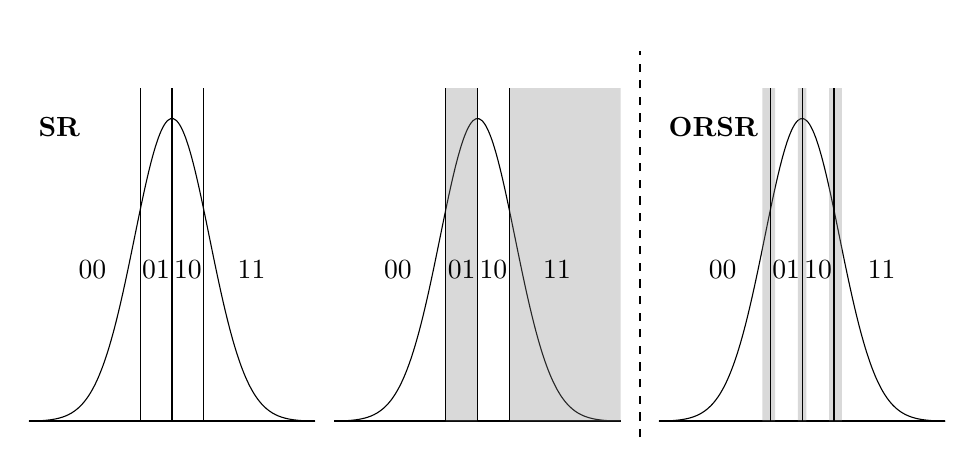
\begin{tikzpicture}
    % -----------------------------------------------------------------
    % --- geometry knobs -----------------------------------------------------------
    \def\axw{0.30\textwidth}  % width of each axis
    \def\gap{0.02\textwidth}  % uniform horizontal gap g
    \def\labely{3.5cm}        % y-position for the group headings (axis height = 5 cm)
    % -----------------------------------------------------------------

    % ----------------------- group headings --------------------------------------
    \node[anchor=south west,font=\bfseries]           at (0,\labely)                    {SR};
    \node[anchor=south west,font=\bfseries]           at ({2*\axw + 3*\gap},\labely)    {ORSR};

    % ----------------------- vertical dashed line --------------------------------
    \draw[thick,dashed]
      ({2*\axw + 2*\gap},-0.2cm) -- ({2*\axw + 2*\gap}, 4.7cm);

    % ----------------------------- Axis 1 ----------------------------------------
    \begin{axis}[
      at={(0,0)}, anchor=south west,
      width=\axw, height=5cm,
      axis lines=middle, domain=-2.8:2.8, samples=100,
      scale only axis, enlargelimits=false,
      ymin=0, ymax=1.3, xmin=-2.7, xmax=2.7,
      xtick=\empty, ytick=\empty,
      x axis line style={thick,-}, y axis line style={draw=none},
    ]
      \addplot[thin,smooth]{exp(-x^2)};
      \draw[thin] (axis cs:-0.6,0) -- (axis cs:-0.6,1.1);
      \draw[thin] (axis cs: 0.0,0) -- (axis cs: 0.0,1.1);
      \draw[thin] (axis cs: 0.6,0) -- (axis cs: 0.6,1.1);
      \node at (axis cs:-1.5,0.5){00};
      \node at (axis cs:-0.3,0.5){01};
      \node at (axis cs: 0.3,0.5){10};
      \node at (axis cs: 1.5,0.5){11};
    \end{axis}

    % ----------------------------- Axis 2 ----------------------------------------
    \begin{axis}[
      at={({\axw+\gap},0)}, anchor=south west,
      width=\axw, height=5cm,
      axis lines=middle, domain=-2.8:2.8, samples=100,
      scale only axis, enlargelimits=false,
      ymin=0, ymax=1.3, xmin=-2.7, xmax=2.7,
      xtick=\empty, ytick=\empty,
      x axis line style={thick,-}, y axis line style={draw=none},
    ]
      \addplot[thin,smooth]{exp(-x^2)};
      \fill[gray,opacity=0.3]
            (axis cs:-0.6,0) rectangle (axis cs:0,1.1)
            (axis cs: 0.6,0) rectangle (axis cs:2.7,1.1);
      \draw[thin] (axis cs:-0.6,0) -- (axis cs:-0.6,1.1);
      \draw[thin] (axis cs: 0.0,0) -- (axis cs: 0.0,1.1);
      \draw[thin] (axis cs: 0.6,0) -- (axis cs: 0.6,1.1);
      \node at (axis cs:-1.5,0.5){00};
      \node at (axis cs:-0.3,0.5){01};
      \node at (axis cs: 0.3,0.5){10};
      \node at (axis cs: 1.5,0.5){11};
    \end{axis}

    % ----------------------------- Axis 3 ----------------------------------------
    \begin{axis}[
      at={({2*\axw + 3*\gap},0)}, anchor=south west,
      width=\axw, height=5cm,
      axis lines=middle, domain=-2.8:2.8, samples=100,
      scale only axis, enlargelimits=false,
      ymin=0, ymax=1.3, xmin=-2.7, xmax=2.7,
      xtick=\empty, ytick=\empty,
      x axis line style={thick,-}, y axis line style={draw=none},
    ]
      \addplot[thin,smooth]{exp(-x^2)};
      \fill[gray,opacity=0.3]
            (axis cs:-0.08,0) rectangle (axis cs:0.08,1.1)
            (axis cs:-0.75,0) rectangle (axis cs:-0.51,1.1)
            (axis cs: 0.51,0) rectangle (axis cs: 0.75,1.1);
      \draw[thin] (axis cs:-0.6,0) -- (axis cs:-0.6,1.1);
      \draw[thin] (axis cs: 0.0,0) -- (axis cs: 0.0,1.1);
      \draw[thin] (axis cs: 0.6,0) -- (axis cs: 0.6,1.1);
      \node at (axis cs:-1.5,0.5){00};
      \node at (axis cs:-0.3,0.5){01};
      \node at (axis cs: 0.3,0.5){10};
      \node at (axis cs: 1.5,0.5){11};
    \end{axis}
    \end{tikzpicture}

    \caption{Comparison of the decoding procedure of multi-round sliced reconciliation (\textbf{SR}) versus the decoding procedure of one-round sliced reconciliation with guard-band post-selection (\textbf{ORSR}). These are compared for reconciling $m = 2$ bits. In the case of SR, multi-stage decoding is performed to first decode the least significant bit (LSB) followed by the most significant bit (MSB). In this example, Alice sends a signal state corresponding to `00', error correction on the LSB allows Bob to exclude areas with LSB = 1 (greyed-out regions) when decoding the MSB. In contrast, ORSR uses guard-bands to rule out regions of probability space (greyed-out regions) via post-selection. This has the benefit of lowering the bit error rate as part of a \textit{single} round of decoding.}

    \label{fig: decoding schematic}
\end{figure*}

We introduce one-round sliced reconciliation with guard-band post-selection. Importantly, one-round sliced reconciliation endeavours to extract $m$ bits in \textit{one} round of error-correction, instead of the $m$ rounds necessary as part of the original theoretical proposal for sliced reconciliation \cite{VanAssche-2004}. This is achieved by quantising Bob's continuous probability space $\mathcal{Y}$ into $2^m$ intervals and assigning each interval a bit string of length $m$. This is analogous to labelling QAM constellation points with Gray or natural binary labels. Due to the information density of the thresholds, \textit{post-selection} may be required to tame the error rates to acceptable levels such that error-correction algorithms can converge \cite{Weerasinghe-2023}. In the same sense that \textit{guard bands} reduce interference between frequency-multiplexed classical communication channels, one-round sliced reconciliation uses guard bands over Bob's probability space $\mathcal{Y}$ to lower the error rate, as is denoted in \figref{fig: decoding schematic}. That is, guard bands filter out Bob's key elements which are considered too likely to be erroneous. The difference in philosophy is clear when we notice that sliced reconciliation multi-round decoding provides interval separation, hence a lower error rate, via multiple stages of error correction. On the other hand, one-round sliced reconciliation provides interval separation via post-selecting around interval boundaries. Operationally, this is just throwing away samples that fall too close to decision boundaries, exactly as in classical receiver designs where samples near thresholds are considered unreliable. These two paradigms are compared in \figref{fig: decoding schematic}.

From a systems engineering standpoint, it is important to note that Bob's key elements are filtered entirely deterministically: they either are within a guard band, or they are not. The post-selection is still probabilistic in the sense that Bob's measurement outcome is \textit{a priori} uncertain, but once measured, the filter is entirely deterministic. Subsequently, the system can deterministically ignore filtered key elements during later key distillation stages.

To introduce formal notions of security, we note that most security analyses in the CV-QKD literature start from the familiar Devetak-Winter equation in the setting where Alice reconciles her key bits against Bob's measurement results -- the so-called reverse-reconciliation scenario \cite{Diamanti-2015, Usenko-2025}. In this scenario, the key efficiency in the asymptotic limit is given by 
\begin{equation}
  \label{eq: K DW}
  K_\infty^\text{DW} = \eta I_{AB} - \chi_{EB}
\end{equation}
where $\eta \in [0, 1]$ is the reconciliation efficiency, $I_{AB}$ is the mutual information between Alice and Bob and $\chi_{EB}$ is the Holevo information between Eve and Bob: the maximum mutual information Eve can extract from her quantum system about Bob's classical data \cite{Devetak-2005}. We can analyse equation \eqref{eq: K DW} further by noticing that Alice produces $H(T(X))$ bits of information from her continuous variable $X \sim \mathcal{N}(0, V_\text{mod})$ after applying her interval quantiser $T : \mathbb{R} \rightarrow \{0, 1\}^m$ \cite{VanAssche-2004, Gray-1998}. Here, $V_\text{mod}$ is the variance of Alice's classical Gaussian modulation in shot-noise units (SNU), i.e. the vacuum noise per quadrature is 1 SNU. As $T(X)$ yields intervals across a Gaussian distribution in the case of GMCS CV-QKD, the probability mass contained in each interval $t_i$ is \cite{VanAssche-2004}
\begin{equation}
  \label{p interval}
  p(t_i) = \frac{1}{2}\left(\text{erf} \left(\frac{\tau_{i+1}}{\sqrt{2V_\text{mod}}}\right) - \text{erf}\left(\frac{\tau_i}{\sqrt{2V_\text{mod}}}\right) \right) \\
\end{equation}
where $V_\text{mod}$ is Alice's modulation variance, $\tau_i$ are the interval thresholds and $\text{erf}(\cdot)$ is the error function. This then naturally leads to $H(T(X)) = -\sum_{i=0}^{2^m - 1} p(t_i) \log_2 p(t_i)$, the Shannon entropy of the quantised variable $T(X)$. 

Upon performing error correction, Alice and Bob leak $\text{LEAK}_{\text{EC}}$ bits of information to Eve. Therefore, the reconciliation efficiency $\eta$ can be defined as
\begin{equation}
  \label{eq: eta}
  \eta = \frac{H(T(X)) - \text{LEAK}_{\text{EC}}}{I_{AB}}
\end{equation}
which is the number of secret bits produced over the theoretical maximum. With this, we can reframe equation \eqref{eq: K DW} as
\begin{equation}
  \label{eq: K full}
  K_\infty = H(T(X)) - \text{LEAK}_{\text{EC}} - \chi_{EB} \\
\end{equation}
which is the key efficiency achievable in the asymptotic limit by Alice and Bob if they choose to reconcile using sliced reconciliation with no post-selection \cite{VanAssche-2004}. We can adapt equation \eqref{eq: K full} to reflect the effect of post-selection on the asymptotic key rate under collective attacks with the use of reverse reconciliation. Defining $p_\text{acc}$ as the probability that a key element is accepted (not discarded) by the post-selection (PS) process,
\begin{equation}
  \label{eq: K ORSR}
  K_{\infty}^\text{PS} = p_\text{acc}\left(H(T(X)) - \text{LEAK}_{\text{EC}}^\text{PS} - \chi_{EB}^\text{PS}\right) \\
\end{equation}
in which $\text{LEAK}_\text{EC}^\text{PS}$ is the publicly leaked information per symbol subject to post-selection, and in which $\chi_{EB}^\text{PS}$ is the focus of the security analysis in \secref{sec: security proof}.

The ultimate measure of a QKD system is its key rate given its security assumptions. In the asymptotic theoretical analysis of CV-QKD systems with post-selection and dual-homodyne detection (therefore two symbols per pulse), the key efficiency can be linearly scaled to the key rate via the system's clock rate $R_\text{clock}$,
\begin{equation}
R_\infty^\text{PS} = 2R_\text{clock}K_\infty^\text{PS}.
\end{equation}
However, this toy model obfuscates trade-offs that can be considered to maximise $R_\infty$. For example, lowering the code rate of the error correcting code increases $\text{LEAK}_\text{EC}$, thereby lowering $K_\infty$. However, doing so may facilitate a higher $R_\text{clock}$ as iterative error-correction algorithms will converge faster. Additionally, the post-selection process reduces the number of key elements available to Alice and Bob, consequently reducing the key efficiency $K_\infty$. However, it also reduces the bit error rate of the key elements that are retained, which can allow for more efficient error correction algorithms to be used, thereby increasing $K_\infty$ and $R_\infty$. For these reasons, a careful balance must be struck between the post-selection probability $p_\text{acc}$ and the error rate $e$. These concepts are explored further in the following subsections.

\subsection{Guard Bands}\label{subsec: guard bands}

Guard band post-selection, first introduced in ref \cite{Weerasinghe-2023} and discussed briefly in \secref{subsec: efficient sliced reconciliation without multi-stage decoding}, is a method of filtering Bob's measurement outcomes to reduce the error rates of the key elements. A graphical representation is given in \figref{fig: decoding schematic}. We can define the guard-band post-selection process using a filter function $F : \mathcal{Y} \rightarrow \{0, 1\}$ such that
\begin{equation}
  \label{eq: F}
F(y) = \begin{cases}
  0 & \text{if } \exists i \in \{0, 1, \ldots, |\mathcal{T}|\}, \text{ such that } -g_{i,-} \leq (y - \tau_i) \leq g_{i,+} \\
  1 & \text{otherwise} \\
\end{cases}
\end{equation}
where $y \in \mathcal{Y}$ is Bob's measurement outcome, and $\mathcal{T} = \{\tau_0,\tau_1,\ldots,\tau_{2^m}\}$ with ordered vector $\boldsymbol{\tau} = (-\infty = \tau_0 < \tau_1 < \cdots < \tau_{2^m-1} < \tau_{2^m} = +\infty)$ denote the slicing thresholds that partition $\mathbb{R}$ into $2^m$ quantised intervals. Finally, $g_{i,-}$ and $g_{i,+}$ are the guard-band extents in the negative and positive directions respectively away from $\tau_i$. That is, if $y$ falls within a guard-band around any threshold, we set $F(y) = 0$ (reject), otherwise the symbol is accepted with $F(y) = 1$. The post-selection probability is then given by
\begin{equation}
  \label{eq: p pass}
  p_\text{acc} = \int_{-\infty}^{\infty} dy \: F(y) p_Y(y) \\
\end{equation}
which is simply the fraction of Bob's samples that survive the post-selection. Proceeding, we find the probability density function of the post-selected variable $Y_\text{PS}$ is given by
\begin{equation}
  \label{eq: p PS}
  p_{Y_\text{PS}}(y) = \frac{F(y)}{p_\text{acc}}p_Y(y) \\
\end{equation}
where division by $p_\text{acc}$ ensures normalisation.

\subsection{Leaked Information and Error Rates}\label{subsec: leaked information and error rates}

\begin{figure*}[t]
  \centering
  \begingroup
  % --------- keep all definitions local to this figure ---------
  % Read data and compute bounds + optimum (all local to this group)
  \pgfplotstableread[col sep=tab]{figure_data/key_efficiency_surface_m2_distance_5km_20x20.dat}\datatable

  % Z stats + argmax
  \pgfplotstablesort[sort key=key_per_pulse, sort cmp=float <]{\tableZ}{\datatable}
  \pgfplotstablegetrowsof{\tableZ}\pgfmathtruncatemacro{\lastZ}{\pgfplotsretval-1}
  \pgfplotstablegetelem{0}{key_per_pulse}\of{\tableZ}\edef\Zmin{\pgfplotsretval}
  \pgfplotstablegetelem{\lastZ}{key_per_pulse}\of{\tableZ}\edef\ZmaxData{\pgfplotsretval}
  \pgfplotstablegetelem{\lastZ}{v_mod}\of{\tableZ}\edef\Xopt{\pgfplotsretval}
  \pgfplotstablegetelem{\lastZ}{p_pass}\of{\tableZ}\edef\Yopt{\pgfplotsretval}
  \pgfplotstablegetelem{\lastZ}{key_per_pulse}\of{\tableZ}\edef\Zopt{\pgfplotsretval}

  % X/Y bounds
  \pgfplotstablesort[sort key=v_mod, sort cmp=float <]{\tableX}{\datatable}
  \pgfplotstablegetrowsof{\tableX}\pgfmathtruncatemacro{\lastX}{\pgfplotsretval-1}
  \pgfplotstablegetelem{0}{v_mod}\of{\tableX}\edef\Xmin{\pgfplotsretval}
  \pgfplotstablegetelem{\lastX}{v_mod}\of{\tableX}\edef\Xmax{\pgfplotsretval}
  \pgfplotstablesort[sort key=p_pass, sort cmp=float <]{\tableY}{\datatable}
  \pgfplotstablegetrowsof{\tableY}\pgfmathtruncatemacro{\lastY}{\pgfplotsretval-1}
  \pgfplotstablegetelem{0}{p_pass}\of{\tableY}\edef\Ymin{\pgfplotsretval}
  \pgfplotstablegetelem{\lastY}{p_pass}\of{\tableY}\edef\Ymax{\pgfplotsretval}

  % --- roof exactly at the top of the axis; generous separation -------------
  \pgfmathsetmacro{\Zrange}{\ZmaxData-\Zmin}
  \pgfmathsetmacro{\Zroof}{\ZmaxData + 1.50*\Zrange} % roof at axis top
  \pgfmathsetmacro{\Zeps}{1e-6} % tiny offset vs. box edges
  \pgfmathsetmacro{\Zroofline}{\Zroof-0.5*\Zeps}

  \begin{tikzpicture}[every node/.style={inner sep=0, outer sep=0}]
    \begin{groupplot}[
      group style={group size=2 by 1, horizontal sep=1.5cm, group name=keygroup},
    ]
      \nextgroupplot[
        width=0.45\textwidth,
        height=0.45\linewidth,
        axis lines=box,
        enlargelimits=false,
        view={-32}{30},
        xmin=\Xmin, xmax=\Xmax,
        ymin=\Ymin, ymax=\Ymax,
        zmin=\Zmin, zmax=\Zroof,
        %
        % --- keep only the "front" ticks/labels; remove top/right ticks -------
        axis on top=false,
        axis line style={on layer=axis background}, % ensures axes drawn first
        xtick pos=lower,
        ytick pos=left,
        ztick pos=left,
        tick align=outside,
        scaled ticks=false,
        tick label style={font=\footnotesize,/pgf/number format/fixed},
        label style={font=\footnotesize},
        title style={font=\footnotesize},
        xlabel={$V_{\mathrm{mod}}$},
        ylabel={$p_{\mathrm{acc}}$},
        ylabel style={rotate=270},
        %zlabel={$K$},
        %
        grid=none,
        colormap/viridis, % back to viridis
        shader=interp,
        z buffer=sort, % draw axes BEFORE surfaces so back edges are occluded (not visible through)
        % i.e. no 'axis on top' here
        point meta min=\Zmin,
        point meta max=\ZmaxData,
        colorbar,              % enable colorbar
        colorbar left,          % <-- this is the right key
        colorbar style={
          width=3mm,
          yticklabel pos=left,
          tick label style={font=\footnotesize,/pgf/number format/fixed, xshift=-3pt}, % add xshift here
          title={$K$},
          title style={font=\footnotesize, yshift=-2pt}, % move title slightly down
        }
      ]
        % --- 3D surface (opaque) ---------------------------------------------
        \addplot3[
          surf, draw=none, mesh/cols=20, point meta=z
        ] table[
          col sep=tab, x=v_mod, y=p_pass, z=key_per_pulse
        ] {\datatable};

        % --- Top projection (opaque heatmap at z = zmax) ---------------------
        \addplot3[
          surf, draw=none, mesh/cols=20, shader=interp, point meta=explicit
        ] table[
          col sep=tab, x=v_mod, y=p_pass, meta=key_per_pulse, z expr=\Zroof-\Zeps
        ] {\datatable};

        % --- Solid guides: up to roof, and over to K-axis corner --------------
        \addplot3[black, very thin] coordinates {(\Xopt,\Yopt,\Zopt) (\Xopt,\Yopt,\Zroof-\Zeps)};
        \addplot3[black, very thin] coordinates {(\Xopt,\Yopt,\Zopt) (\Xmin,\Ymax,\Zopt)};

        % --- Dashed beams from ROOF dot to walls, then down to axes -----------
        % to p_acc/K wall (x = Xmin), then straight down to p_acc axis (z = Zmin)
        \addplot3[black, dashed, very thin] coordinates {(\Xopt,\Yopt,\Zroofline) (\Xmin,\Yopt,\Zroofline)};
        \addplot3[black, dashed, very thin] coordinates {(\Xmin,\Yopt,\Zroofline) (\Xmin,\Yopt,\Zmin)};
        % to V_mod/K wall (y = Ymin), then straight down to V_mod axis (z = Zmin)
        \addplot3[black, dashed, very thin] coordinates {(\Xopt,\Yopt,\Zroofline) (\Xopt,\Ymin,\Zroofline)};
        \addplot3[black, dashed, very thin] coordinates {(\Xopt,\Ymin,\Zroofline) (\Xopt,\Ymin,\Zmin)};

        % --- Peak markers (white dots with black border) ----------------------
        \addplot3[
          only marks, mark=*, mark size=1.8pt, draw=black, fill=white
        ] coordinates {(\Xopt,\Yopt,\Zopt)};
        \addplot3[
          only marks, mark=*, mark size=1.8pt, draw=black, fill=white
        ] coordinates {(\Xopt,\Yopt,\Zroof-\Zeps)};

      \nextgroupplot[
        name=optimalparamsGroup,
        width=0.35\textwidth,
        height=0.3\textwidth,
        scale only axis,
        tick label style={font=\small,/pgf/number format/fixed},
        label style={font=\small},
        tick align=outside,
        tick style={semithick},
        axis y line*=left,
        axis x line*=bottom,
        xmin=0, xmax=30,
        ymin=0, ymax=5.1,
        enlarge y limits={upper=0.02},
        enlarge x limits=false,
        xtick distance=5,
        minor x tick num=1,
        xlabel={Distance (km)},
        xlabel near ticks,
        xlabel shift=5pt,
        %ylabel={Optimal $V_{\text{mod}}$},
        % --- STANDARDIZED label spacing (left)
        ylabel near ticks,
        ylabel shift=-10pt,                  % fixed gap from tick labels
        ylabel style={text=blue!70!black}, % color only
        % in the blue (left‑y) axis options of the right-hand figure:
        y tick label style={text=blue!70!black, xshift=-3pt},
        xmajorgrids,                       % no grid lines
        grid=none,
        line cap=round, line join=round,
      ]
        \addplot+[line width=1.05pt, mark=none, color=blue!70!black]
          table[col sep=tab, x=distance_km, y=optimal_v_mod]
            {figure_data/optimal_params_m2_distance_upto_30km.dat};
    \end{groupplot}

    % --- Right axis: p_acc overlay on second group plot column ---------------
    \begin{axis}[
      width=0.35\textwidth,
      height=0.3\textwidth,
      at={(optimalparamsGroup.south west)}, anchor=south west,
      scale only axis,
      tick label style={font=\small,/pgf/number format/fixed},
      tick align=outside,
      tick style={semithick},
      axis x line=none,
      axis y line*=right,
      xmin=0, xmax=30,
      ymin=0, ymax=1.02,                 % tiny headroom for the "1"
      ytick={0.2,0.4,0.6,0.8,1.0},
      yticklabel pos=right,
      % ylabel={Optimal $p_\text{acc}$},
      % --- STANDARDIZED label spacing (right)
      ylabel near ticks,
      %ylabel shift=8pt,                  % same fixed gap as left
      ylabel style={text=red!70!black},
      y tick label style={text=red!70!black, xshift=3pt}, % keep clear of the "30"
      legend pos=north east,
      legend style={draw=none, fill=none, font=\small},
      legend cell align=left,
    ]
      \addlegendimage{line width=1.05pt,color=blue!70!black}
      \addlegendentry{Optimal $V_{\text{mod}}$}

      \addplot+[line width=1.05pt, mark=none, color=red!70!black, densely dashed]
        table[col sep=tab, x=distance_km, y=optimal_p_pass]
          {figure_data/optimal_params_m2_distance_upto_30km.dat};
      \addlegendentry{Optimal $p_\text{acc}$}
    \end{axis}
  \end{tikzpicture}
  \endgroup
  % --------- end local scope --------------------------------------
  \caption{Left: Key efficiency surface $K$ as a function of both the modulation variance $V_\text{mod}$ and the acceptance rate of the post-selection $p_\text{acc}$ for a fibre transmission distance of 5 km with a loss coefficient of 0.2 dB/km, excess noise of 0.001 SNU, and the reconciliation of $m = 2$ bits per symbol. The optimum point is highlighted by a white dot, and the dashed lines indicate its projections onto the optimal parameters $V_{\mathrm{mod}}$ and $p_{\mathrm{acc}}$. This is a classical link-budget style trade-off: more modulation increases SNR but also boosts Eve's information; more aggressive guard bands reduce error rate but discard more symbols. Right: Similarly, the optimal $V_\text{mod}$ and $p_\text{acc}$ that maximise the key efficiency $K$ as a function of fibre transmission distance, from 1 km to 30 km. Note that the optimal $p_\text{acc}$ decreases with distance as expected, reflecting that the channel becomes noisier over distance.}
  \label{fig:key_efficiency_surface_group}
\end{figure*}

Importantly, Alice and Bob must quantify the amount of relevant classical information $\text{LEAK}_{\text{EC}}$ communicated publicly over their classical channel. After post-selection, Alice and Bob can, in principle, take an information-theoretically optimal approach and only communicate $H(T(X)|T(Y_\text{PS}))$ bits to recover a shared identical key \cite{VanAssche-2004, Slepian-1973}. That is, they've recovered 
\begin{equation}
  \label{eq: I AB PS}
I_{AB}^\text{PS} = I(T(X); T(Y_\text{PS})) = H(T(X)) - H(T(X)|T(Y_\text{PS}))
\end{equation}
bits of mutual information per accepted symbol. Via the chain rule of mutual information, it is easy to show that post-selection does not increase Alice and Bob's shared mutual information:
\begin{equation}
  \label{eq: MI proof}
  p_\text{acc} I_{AB}^\text{PS} = p_\text{acc} I(T(X); T(Y) | F(Y) = 1) \leq I(T(X);T(Y)).
\end{equation}
That is, post-selection does not increase the per-channel-use mutual information between Alice and Bob. However, we will see that post-selection can provide a more favourable bound on Eve's information, as will be discussed in \secref{sec: security proof}. More importantly, post-selection is also favourable when trying to reconcile $I(T(X); T(Y))$ in practice with effective binary channels \cite{Heid-2007, Silberhorn-2002}. That is, post-selection improves the reconciliation efficiency $\eta_\text{PS}$ because the effective signal-to-noise ratio (SNR) increases on the accepted symbols, leading to lower bit error rates. Therefore, $p_\text{acc}\eta_\text{PS} I_{AB}^\text{PS}$ can still outperform $\eta I(T(X); T(Y))$ with practical error-correcting codes \cite{Weerasinghe-2023}. Clearly, trade-offs between information theory and practical implementation must be made to bolster the achievable key rate.

We first turn our attention to the illustrative case of reconciling $m = 1$ bit per symbol. In this case, Bob's probability space $\mathcal{Y}$ is partitioned into two intervals separated by a single finite threshold $\tau_1 = 0$. This allows us to model the channel as a binary symmetric channel (BSC) with capacity $C_\text{BSC} = 1 - h_2(e)$ where $e$ is the bit error rate and $h_2(\cdot)$ is the binary Shannon entropy \cite{Cover-2006}. Here $e$ is the bit error rate of the effective binary channel obtained after slicing and post-selection. With a coding efficiency $\eta_c(e)$ as a function of error rate $e$ in practice, the channel coding rate is therefore
\begin{equation}
  \label{eq: R_c}
  R_c(e) = \eta_c(e)C = \eta_c(e)(1 - h_2(e))
\end{equation}
such that the leaked information per symbol is 
\begin{equation}
\label{eq: LEAK EC}
\text{LEAK}_\text{EC} = m(1 - R_c(e)) = m(1 - \eta_c(e)(1 - h_2(e))).
\end{equation}
In latency-aware environments such as in high-rate CV-QKD systems, the coding efficiency $\eta_c(e)$ is a function parameterised by the chosen minimum decoding speed $S_\text{min}$ (in bits per second) such that
\begin{equation}
\label{eq: eta_c e Smin}
\eta_c(e; S_\text{min}) = \frac{R_c(e; S_\text{min})}{C_\text{BSC}} \leq 1
\end{equation}
such that $R_c$ (and $\eta_c$) are therefore highly implementation dependent \cite{Weerasinghe-2023}. For a fixed LDPC design and decoder speed budget $S_\text{min}$, $\eta_c$ summarises how close one can operate to Shannon capacity at each error rate.

We now return to the case of reconciling general $m$ bits per symbol. In this case, the channel between Alice and Bob is no longer a BSC (however the process of slicing with multi-stage decoding recovers $m$ effective BSCs \cite{VanAssche-2004}). In practice, whether using multi-stage decoding or one-round decoding, soft information in the form of log-likelihood ratios is often used with low-density parity-check (LDPC) codes to improve error-correction performance to near capacity-achieving \cite{Yang-2023a}. To remain agnostic with respect to the specific coding scheme used, we return to the Slepian-Wolf theorem which states that Alice and Bob need only leak $H(T(X)|T(Y_\text{PS}))$ bits per accepted symbol to reconcile their keys (noting that this reduces to $h_2(e)$ for $m = 1$) \cite{Slepian-1973}. Modelling the coding overhead as a function of $m$, we can write
\begin{equation}
  \label{eq: LEAK EC general m}
  \text{LEAK}_\text{EC}^\text{PS} = (1 + \epsilon)H(T(X)|T(Y_\text{PS}))
\end{equation}
with $\epsilon \geq 0$ being a small coding inefficiency parameter \cite{VanAssche-2004}. With some algebra, we find that the efficiency with which information can be reconciled from $T(X)$ becomes
\begin{equation}
  \label{eq: eta SW}
  \eta^\text{PS}_{T(X)} = 1 - \frac{\epsilon H(T(X)|T(Y_\text{PS}))}{I_{AB}^\text{PS}}.
\end{equation}

\section{Security Analysis}\label{sec: security proof}

Our goal is to upper bound Eve's Holevo information $\chi_\Phi(E;U|F)$ without assuming that the effective state after guard-band post-selection is Gaussian. We proceed in three conceptual steps. We first compute a reference bound $\chi_\mathcal{G}(E;U|F)$ under the Gaussian channel model $\mathcal{G}(T,\xi)$ determined by the estimated transmissivity $T$ and excess noise $\xi$, using Gaussian optimality and covariance-matrix methods. Because our protocol is continuous-variable, the underlying Hilbert spaces are infinite-dimensional. Therefore, secondly, we introduce a photon number cutoff $N$ and certify (operationally) that the probability weight outside the truncated Fock subspace is small by performing an energy test on a randomly chosen subset of rounds. Conditioned on passing the test, the outside-cutoff weight is bounded by a parameter $W \le w$ except with probability $\varepsilon_{\mathrm{test}}$. This allows us to rigorously reduce the security analysis to a finite-dimensional subspace at the cost of an explicit, quantified penalty. Thirdly, we with to remain compatible with Gaussian optimality arguments. Therefore, within the truncated space, we quantify the deviation between the true channel $\Phi$ and the Gaussian channel model $\mathcal{G}$ via a protocol-specific state distance $\varepsilon_{\Phi \mathcal{G}}$ between the corresponding entanglement-based states. Using Uhlmann's theorem, we `lift' this reduced-state distance to a distance between suitable purifications that include Eve's system, and then proceed to use the contractivity of trace distance under Bob's classical post-processing map to obtain a bound on the distance between the resulting classical-quantum (cq) states shared by Eve and Bob's classical registers. Finally, we apply tight continuity bounds for cq entropies to convert this small cq-state distance into an explicit additive correction to the Gaussian-derived key efficiency term, yielding a continuity-corrected upper bound on $\chi_\Phi(E;U|F)$ that covers general collective attacks compatible with the energy test.

\subsection{Gaussian Optimality}\label{subsec: gaussian optimality}

The security analysis of a QKD protocol is ultimately the pursuit of an upper bound for the amount of information available to Eve from her quantum-mechanical attacks (the Holevo information, $\chi$, which in our context is $\chi_{EB}$ between Eve and Bob), given a set of assumptions about the capabilities of Eve. In classical terms, we are upper-bounding Eve's mutual information with Bob's data, under specific assumptions about her physical capabilities. In our case, we need to deal with Eve potentially making use of the guard-band post-selection procedure to gain information. The security of post-selection as part of a CV-QKD protocol has seen extensive prior study \cite{Fiurasek-2012, Walk-2013, Hosseinidehaj-2020, Heid-2007, Heid-2006, Silberhorn-2002, Blandino-2012}. However, rather than showing that the resulting \textit{state} after post-selection is compatible with security proofs based on Gaussian optimality, we rely on a set of probe and measurement settings that fully characterise the quantum channel to ensure that the \textit{channel} between Alice and Bob is Gaussian (to a close enough approximation) such that entropic continuity results (continuity of entropy with respect to small changes in the underlying channel) can be invoked to then apply Gaussian optimality.

Gaussian optimality refers to the principle that Gaussian quantum states provide extremal values for entanglement measures and entropies in the set of continuous-variable quantum states \cite{Wolf-2006}. Subsequently, they provide an optimal distillable secret key efficiency $K$ \cite{Wolf-2006}. For constant first and second statistical moments of Alice and Bob's shared state $\rho_{AB}$,
\begin{equation}
\label{eq: gaussian optimality}
K(\rho_{AB}) \geq K^\text{Gaussian}(\rho_{AB})
\end{equation}
such that Eve's optimal attack against a Gaussian-modulated CV-QKD protocol is one that introduces Gaussian noise and loss across the quantum channel -- a \textit{Gaussian attack} \cite{Garcia-Patron-2006, Navascues-2006}. That is, among all states that share the same first and second moments (covariance matrix), the Gaussian state is the worst case for the key rate. Compared to other security proofs, security proofs based on Gaussian optimality are mature, well-rounded and operational \cite{Usenko-2025}. When considering the security of the GMCS CV-QKD protocol with guard-band post-selection using the Gaussian optimality, a problem arises -- Bob's statistics are no longer Gaussian. Therefore, in the entanglement-based picture, the effective state shared between Alice and Bob $\rho_{AB}$ is no longer Gaussian. Can Eve infiltrate the system by exploiting this? She would need to do so by performing a technologically-challenging subtle non-Gaussian attack (i.e. an operation that does more than simply add Gaussian noise and loss, such as photon addition) that still produces the covariance matrix that Alice and Bob measure \cite{Usenko-2025}.

Even given these non-Gaussian statistics, Alice and Bob may still construct an effective covariance matrix with their measured second moments of their non-Gaussian data to achieve a loose bound on $\chi_{EB}$ using Gaussian optimality. However, the bound becomes looser as Bob's statistics stray further from the Gaussian regime, and it quickly becomes prohibitive. As an alternative, Alice and Bob can simply assume Gaussian collective attacks only, therefore waiving security against general collective attacks \cite{Heid-2007}. Although, this is an unsatisfying assumption as the gold-standard in the analysis of GMCS CV-QKD protocols is security in the face of arbitrary collective attacks \cite{Diamanti-2015}.

Not wishing to assuming Gaussian attacks, can Alice and Bob attempt to use different arguments, not necessarily Gaussian optimality, to bound $\chi_{EB}$? Semi-definite programming techniques applied to discrete-modulated CV-QKD protocols are unfortunately computationally intractable for constellations higher than 64-QAM \cite{Ghorai-2019} (our Gaussian modulation has an effective discretised constellation size of order $10^4$ due to the two 8-bit A2D cards used, see ref. \cite{Weerasinghe-2023}).

Therefore, for the security analysis presented here, we turn to the use of Gaussian optimality arguments even though $\rho_{AB}$ is no longer Gaussian after guard-band post-selection. We first start with Gaussian optimality to find a bound on $\chi_{EB}$. The trick is to then alleviate the Gaussian attack assumption with quantum channel estimation. Alice and Bob must then formally account for this step in the security analysis by exploiting entropic continuity arguments. The characterisation of the quantum channel between Alice and Bob can be efficiently undertaken using the procedure outlined in \appref{app: channel estimation with cv-qkd data}. Operationally, this is just using the same data that Alice and Bob use for parameter estimation but treating it as training data for a channel model.

\subsection{Eve's Information under a Gaussian Channel}\label{subsec: eves information}

Following the discussion above, we first consider that the quantum channel shared by Alice and Bob is a Gaussian one, $\mathcal{G}(T, \xi)$ with transmissivity $T$ and excess noise $\xi$ (the same $T$ and $\xi$ estimated from the prepare-and-measure picture in \figref{fig: modulation schematic}). Eve's information when she is capable of a Gaussian attack is completely determined by $\mathcal{G}$ and Alice's modulation variance $V_\text{mod}$, where both $\xi$ and $V_\text{mod}$ are expressed in shot-noise units (see \figref{fig: modulation schematic}).

In the reverse reconciliation scenario (Bob's received key elements form the key, rather than Alice's sent elements), Eve's information is given by
\begin{equation}
\chi(E;U|F)
\end{equation}
which is the Holevo information between Eve's quantum system $E$ and Bob's classical post-processed symbol $U$, conditioned on the post-selection flag $F$. Here, $U$ is Bob's classical symbol after quantisation and post-selection, and $F$ is a flag indicating whether the symbol was kept or discarded. For classical registers (ordinary classical random variables), the chain rule for the Holevo information gives
\begin{equation}
  \chi(E;U|F) = \chi(E;UF) - \chi(E;F)
\end{equation}
where the first term $\chi(E;UF)$ is Eve's information about both Bob's symbol \textit{and} whether it was accepted or rejected, and the second term $\chi(E;F)$ subtracts off information carried by the flag alone. We define $U$ such that for rejected events $(F = 0)$, Bob outputs a fixed dummy variable (such as $U = \bot$); hence $U$ carries no information conditional on $F = 0$, and all information relevant to Eve is in $U|F=1$. This ensures that rejected symbols carry no extra information about Alice's input, so we can cleanly factor them out of Eve's information. Therefore,
\begin{equation}
  \chi(E;U|F) = p_\text{acc} \chi(E;J|\text{acc})
\end{equation}
where $p_\text{acc} = p(F = 1)$ (see equation \eqref{eq: p pass}) and $J$ is the classical variable obtained by Bob after his dual-homodyne measurement and quantisation \textit{conditioned on acceptance} by the guard-band post-selection procedure. So, $\chi(E;J|\text{acc})$ is the quantity that directly affects the key bits we actually keep. As we know the form of $p_\text{acc}$ from equation \eqref{eq: p pass}, our task is to now compute $\chi(E;J|\text{acc})$ subject to $\mathcal{G}(T, \xi)$.

The initial step is a standard `purification' argument: we mathematically attribute all loss and noise in the Alice-Bob channel to an environment held by Eve such that Eve's system purifies the joint state $\rho_{AB}$ shared between Alice and Bob \cite{Laudenbach-2018}. With this, we can express $\chi$ as
\begin{equation}
\label{eq: chi EB von Neumann}
\chi = S(AB) - S(A|\beta) = S(E) - S(E|\beta)
\end{equation}
in which $S(AB)$ is the von Neumann entropy of Alice and Bob's effective joint state and $S(A|\beta)$ is the von Neumann entropy of Alice's state conditioned on Bob's dual-homodyne measurement result $\beta = (y_1 + i y_2)/2$ in shot-noise units (so $\beta$ is a complex number whose real and imaginary parts are Bob's two quadrature measurements, see \appref{app: universal purification analysis} for further details).

The Holevo information $\chi$ is straightforwardly calculated using Gaussian optimality for continuous outcomes, which can serve as a loose upper bound (see \appref{app: covariance matrices and holevo information}). We must now adapt this to account for Bob's quantisation to a classical register. For this, it is convenient to write the joint state of Eve and Bob's classical register as a \textit{classical-quantum} state (cq-state): a \textit{classical} label $j$ stored in Bob's register and a possibly-correlated corresponding \textit{quantum} state held by Eve. We now package `Bob chooses interval $j$' and `Eve holds the corresponding quantum state' into a single cq-state. This ultimately is just bookkeeping to match the standard definition of the Holevo quantity. Considering Bob's classical register $J$ obtained after his dual-homodyne measurement, quantisation and guard-band post-selection, we can define the accepted cq-state as
\begin{equation}
  \rho_{EJ}^\text{acc} = \sum_j p_{j|\text{acc}} \rho_E^{(j,\text{acc})} \otimes |j\rangle\langle j|
\end{equation}
where the state for a given quantisation interval $j$ is
\begin{equation}
\rho_E^{(j,\text{acc})} = \frac{1}{p_{j|\text{acc}}} \int_{\beta \in J_j} p(\beta) \rho_E^\beta d\beta.
\end{equation}
That is, $\rho_E^{(j,\text{acc})}$ is the average of Eve's conditional states over all dual-homodyne outcomes $\beta$ that fall into Bob's accepted interval $J_j$. Following the standard definition of the Holevo information for cq-states \cite{Watrous-2018}, we find that the Holevo information per accepted symbol is
\begin{equation}
  \label{eq: chi EB post-selection}
  \chi(E;J|\text{acc}) = S(E|\text{acc}) - \sum_j p_{j|\text{acc}} S\left(\rho_E^{(j,\text{acc})}\right).
\end{equation}
Subject to the strictly Gaussian channel $\mathcal{G}(T, \xi)$, we find that Eve's states $\rho_E^\beta$ are Gaussian states displaced over $\beta$ phase space with a $\beta$-independent covariance matrix $\Sigma_{E|\beta}$. We may use Gaussian optimality to evaluate the first term in equation \eqref{eq: chi EB post-selection} \cite{Navascues-2006}. Intuitively, among all states with a fixed covariance matrix, a Gaussian state has the largest entropy. For the second (conditional) term, we may use the concavity of the von Neumann entropy with the fact that conditional Gaussian states $\rho_E^\beta$ share the same covariance matrix and hence the same entropy \cite{Nielsen-2010}. Applying these two results, we find that the accepted register Holevo information is upper bounded by
\begin{equation}
\chi_\mathcal{G}(E;J|\text{acc}) \leq S(\Sigma_E^\text{acc}) - S(\Sigma_{E|\beta})
\end{equation}
where $S(\Sigma)$ denotes the von Neumann entropy of a Gaussian state with covariance matrix $\Sigma$ (computed via its symplectic eigenvalues, see \appref{app: covariance matrices and holevo information}). Thus, \textit{under the Gaussian reference channel} Eve's information after guard bands is determined fully by two covariance matrices: one for her conditional state given Bob's outcome, and one for her state after we average over the accepted outcomes. The matrix $\Sigma_E^\text{acc}$ has the form
\begin{equation}
  \Sigma_E^\text{acc} = \Sigma_{E|\beta} + M \text{cov}(\beta|\text{acc})M^T, \quad M = \Sigma_{EB}(\Sigma_B + \mathbb{I}_2)^{-1},
\end{equation}
more details about which are given in \appref{app: covariance matrices after post-selection}. The matrix $\text{Cov}(\beta|\text{acc})$ is simply the covariance matrix of Bob's complex dual-homodyne outcomes $\beta$ conditioned on the event that $\beta$ passes the guard-band post-selection. We also use this quantity to compute Bob's mutual information in \secref{sec: one-round sliced reconciliation with guard bands}. With this, we have reached an upper bound on Eve's information per channel use subject to a Gaussian channel $\mathcal{G}(T, \xi)$ and guard-band post-selection:
\begin{equation}
  \label{eq: final gaussian bound}
  \boxed{\chi_\mathcal{G}(E;U|F) = p_\text{acc} \chi_\mathcal{G}(E;J|\text{acc}) \leq p_\text{acc} \left(S(\Sigma_E^\text{acc}) - S(\Sigma_{E|\beta})\right).}
\end{equation}
In words: under a Gaussian (AWGN) channel $\mathcal{G}(T,\xi)$, we can bound Eve's information after guard-band post-selection purely from the covariance matrices of Alice, Bob and Eve's conditional states.

\subsection{Finite Dimensions}
\label{subsec: Finite Dimensions}

As introduced, we do not wish to assume that the true attack implemented by Eve is Gaussian. Instead, as in the last section, we compute a `base' value for the Holevo information considering the Gaussian channel model $\mathcal{G}(T, \xi)$. This `base' Eve term in the post-selection regime is calculated using Gaussian optimality arguments as outlined in the previous subsection. We propose that Alice and Bob are able to use quantum channel estimation with an energy-test achieve a raised bound on the Holevo information using continuity corrections, but a bound within which it is safe to perform post-selection. In this section and those to follow, we detail the computation of this bound.

Noting that Alice and Bob are implementing a continuous-variable protocol, we let $\mathcal{H}^{A}$ and $\mathcal{H}^{B}$ be separable, infinite-dimensional Hilbert spaces associated with Alice and Bob respectively. Between them is their completely positive and trace-preserving (CPTP) channel $\Phi: \mathcal{L}(\mathcal{H}^{A}) \mapsto \mathcal{L}(\mathcal{H}^{B})$, i.e. the mathematical representation of the physical optical channel between Alice and Bob. Here, $L(H)$ denotes the set of bounded linear operators on the Hilbert space $H$ (matrices acting on the state space). Alice and Bob must perform calculations in a finite-dimensional subspace of $\mathcal{H}^{A}$ and $\mathcal{H}^{B}$ to avoid mathematical complications associated with infinite-dimensional spaces (see \appref{app: channel estimation with cv-qkd data}) \cite{Lobino-2008, Rahimi-Keshari-2011}. Fixing a photon number cutoff $N$, we define the number projector onto the first $N + 1$ Fock levels as
\begin{equation}
\label{eq: number projector}
\Pi_N=\sum_{n=0}^N\ket{n}\bra{n}
\end{equation}
such that Alice and Bob enjoy the finite subspaces $\mathcal{H}_N^{A} = \Pi_N \mathcal{H}^{A}$ and $\mathcal{H}_N^{B} = \Pi_N \mathcal{H}^{B}$. In practice this corresponds to restricting attention to states with at most $N$ photons in the optical mode, which is reasonable given that we know Alice's finite modulation variance in advance. Alice and Bob, for now, will perform their channel reconstruction on $\mathcal{H}_N^{A}$ and $\mathcal{H}_N^{B}$, and in doing so will recover the truncated channel $\Phi_N$ (see \appref{app: channel estimation with cv-qkd data}) which is to be compared to the truncated Gaussian channel $\mathcal{G}_N$:
\begin{equation}
\label{eq: truncated channel}
\Phi_N(X) = \Pi_N \Phi(\Pi_N X \Pi_N) \Pi_N, \quad \mathcal{G}_N(X) = \Pi_N \mathcal{G}(\Pi_N X \Pi_N) \Pi_N.
\end{equation}

\subsection{Energy Testing and Dimension Reduction}
\label{subsec: energy test}

Similar security proofs have also not relied on Gaussian optimality, but have instead relied on finite-energy constraints to limit Eve's capabilities \cite{Kaur-2021}. To address this in our protocol, we use an \textit{energy test} to operationally certify that Bob's received states have negligible support outside of the finite-dimensional subspace $\mathcal{H}_N^{B}$. 

To this end, we can adopt similar energy tests developed for the analysis of discrete-modulated CV-QKD protocols \cite{Kanitschar-2023}. Also adopting the notation of ref \cite{Kanitschar-2023}, Bob randomly selects $k_T$ test rounds, similarly to the parameter estimation rounds of a CV-QKD protocol. On these rounds, he examines the magnitude of his dual-homodyne detection outcomes and compares this value with some threshold $\beta_\text{test}^2$. The energy test passes if at most $l_T$ of the $k_T$ test rounds exceed $\beta_\text{test}$, otherwise, the energy test fails and the protocol aborts.

Defining the in-subspace weight $W$ of Bob's received state $\rho_B^\Phi$, we wish to perform a statistical test such that $W$ is bounded by some security-relevant weight parameter $w$: 
\begin{equation}
  \label{eq: W}
  W = \text{Tr} \left[\left(\mathbb{I} - \Pi_N\right) \rho_B^\Phi \right] \leq w.
\end{equation}
Following theorem 2 of ref \cite{Kanitschar-2023}, we find that, if the energy test passes, then $W \leq w$ with probability at least $1 - \varepsilon_\text{test}$. Of course, $\varepsilon_\text{test}$ is small a security parameter which is a function of the security demands of the system, and therefore should be parameterised accordingly in terms of $\beta_\text{test}$, $w$, $N$, $k_T$, $l_T$, etc, as within ref \cite{Kanitschar-2023}.

With the finite-dimensional subspaces defined and the energy test in place, we may now use the recently-developed \textit{dimension reduction} technique of ref \cite{Upadhyaya-2021}. This technique formalises the extent to which the achievable secure key rate should be punished due to the restriction of Alice and Bob's analysis to finite dimensions. That is, it allows CV-QKD protocols employing a photon number cutoff assumption to relax this assumption at the cost of a small key rate penalty. Adapting Lemma 1 of ref \cite{Upadhyaya-2021}, we can define a convenience function
\begin{equation}
  \label{eq: kappa}
  \kappa(\varepsilon, |Z|) = \varepsilon \log_2 |Z| + (1 + \varepsilon) h_2\left(\frac{\varepsilon}{1 + \varepsilon}\right).
\end{equation}
where $|Z|$ is the dimension of the key map register, with $|Z| = 2^m$ for an $m$-bit key map as in the case of (one-round) sliced reconciliation. The function $\kappa(\varepsilon,|Z|)$ is an Alicki-Fannes type uniform continuity bound for conditional entropies of cq-states \cite{Winter-2016}. That is, if quantum states $\rho_{ZE}$ and $\sigma_{ZE}$ are classical on $Z$ with alphabet size $|Z|$ and satisfy $\tfrac12\|\rho_{ZE}-\sigma_{ZE}\|_1\le \varepsilon$, then \cite{Winter-2016}
\begin{equation}
\big|H(Z|E)_\rho - H(Z|E)_\sigma\big| \le \kappa(\varepsilon,|Z|).
\end{equation}
Crucially, this bound depends only on the classical alphabet size $|Z|$ and not on $\dim(E)$. Then, with Theorem 2 of \cite{Upadhyaya-2021}, the key rate penalty due to dimension reduction is
\begin{equation}
  \label{eq: dimension reduction penalty}
  \Delta(W) = \kappa(\varepsilon_W, |Z|) \text{ with } \varepsilon_W = \sqrt{2W - W^2}.
\end{equation}

\subsection{Channel and State Distances}
\label{subsec: channel and state distances}

Now that we have permitted the security analysis to consider finite dimensions only, and quantified the punishment incurred to do so, we may now consider how close the true channel $\Phi$ is to the Gaussian channel model $\mathcal{G}$ in order to continue alleviating the Gaussian attack assumption. To this end, it is convenient to equivalently consider Alice and Bob's states instead of the channel itself, and to work in the entanglement-based picture. Alice retains a reference mode $A$, and transmits a mode $A'$ through the channel to Bob, who receives mode $B$. Subsequently, the shared state between Alice and Bob is
\begin{equation}
  \rho_{AB}^{\Phi} = (\mathrm{id}_A\otimes \Phi)(|\psi\rangle\langle\psi|_{AA'})
\end{equation}
and similarly for the Gaussian channel $\mathcal{G}$ we have
\begin{equation}
  \rho_{AB}^{\mathcal{G}} = (\mathrm{id}_A\otimes \mathcal{G})(|\psi\rangle\langle\psi|_{AA'})
\end{equation}
where $|\psi\rangle_{AA'}$ is the two-mode squeezed vacuum (TMSV) state that Alice would prepare in the entanglement-based picture \cite{Laudenbach-2018}. Imposing the photon number cutoff $N$ as before, we may define the (renormalised) truncated states $\rho_{AB}^{\Phi,N}$ and $\rho_{AB}^{G,N}$ supported on $\mathcal H_A^N\otimes \mathcal H_B^N$. We can then define the trace distance between these two states to be 
\begin{equation}
\label{eq: trace distance}
\varepsilon_{\Phi \mathcal{G}} = \tfrac{1}{2}\left\|\rho_{AB}^{\Phi,N}-\rho_{AB}^{G,N}\right\|_1
\end{equation}
which is an efficiently computable state distance measure \cite{Watrous-2018}.

However, we have only bounded the distance between the reduced (truncated) states on $AB$. To relate this to Eve's system, we may assume without loss of generality that Eve holds a purification of Alice and Bob's joint state. That is there exist purifications $\rho^{\Phi,N}_{ABE}$ and $\rho^{G,N}_{ABE}$ of $\rho^{\Phi,N}_{AB}$ and $\rho^{G,N}_{AB}$, respectively, on a common Hilbert space that includes Eve (see \appref{app: universal purification analysis}).

By Uhlmann's theorem and the Fuchs--van de Graaf inequalities \cite{Watrous-2018}, one can choose these purifications
such that their trace distance is controlled by a reduced-state trace distance $\varepsilon_\text{pur}$ that is a simple function of $\varepsilon_{\Phi \mathcal{G}}$:
\begin{equation}
\label{eq: purification distance}
\varepsilon_{\rm pur}
=\sqrt{2\varepsilon_{\Phi G}-\varepsilon_{\Phi G}^2}
\le \sqrt{2\varepsilon_{\Phi G}},
\end{equation}
such that
\begin{equation}
\label{eq: Eve state distance}
\tfrac{1}{2}\left\|\rho_{ABE}^{\Phi,N}-\rho_{ABE}^{G,N}\right\|_1 \le \varepsilon_{\rm pur}.
\end{equation}

Letting $C$ denote Bob's classical post-processing map (dual-homodyne measurement, slicing, and the guard-band acceptance flag) whose outputs are the classical registers $U$ and $F$ as within equation \eqref{eq: final gaussian bound}. Applying $C$ to Bob's system and tracing out Alice's system cannot increase trace distance \cite{Watrous-2018}, so by contractivity under completely-positive trace-preserving maps we obtain the cq-state distance bound
\begin{equation}
\label{eq: Eve-Bob cq-state distance}
\tfrac{1}{2}\left\|\rho_{EUF}^{\Phi,N}-\rho_{EUF}^{G,N}\right\|_1 \le \varepsilon_{\rm pur}.
\end{equation}
Therefore, the distance by which Eve's cq-states are removed from those induced by the Gaussian channel model is completely quantified by the computable quantity $\varepsilon_{\Phi \mathcal{G}}$.

\subsection{Continuity Corrections and Final Key Rate}
\label{subsec: continuity corrections and final key rate}

The task now becomes translating the computed Eve's cq-state distance into a bound on the difference in Holevo information $\chi(E;U|F)$ between the true channel $\Phi$ and the Gaussian model $\mathcal{G}$. Letting $\rho_{EUF}^\Phi$ and $\rho_{EUF}^G$ be the true (infinite-dimensional) cq-states produced by the protocol under $\Phi$ and $\mathcal{G}$, respectively, and letting the superscript $N$ denote the truncated versions. By inserting the cq-states and applying the triangle inequality we find that
\begin{align}
  \label{eq: long one}
\tfrac12\|\rho^\Phi_{EUF}-\rho^G_{EUF}\|_1
&=\tfrac12\|(\rho^\Phi_{EUF}-\rho^{\Phi,N}_{EUF})+(\rho^{\Phi,N}_{EUF}-\rho^{G,N}_{EUF})
+(\rho^{G,N}_{EUF}-\rho^G_{EUF})\|_1 \nonumber\\
&\le \tfrac12\|\rho^\Phi_{EUF}-\rho^{\Phi,N}_{EUF}\|_1
+ \tfrac12\|\rho^{\Phi,N}_{EUF}-\rho^{G,N}_{EUF}\|_1
+ \tfrac12\|\rho^{G,N}_{EUF}-\rho^G_{EUF}\|_1.
\end{align}
We may then define the truncation errors
\begin{equation}
\varepsilon_{\mathrm{trunc}}^{\Phi} = \frac12\|\rho^\Phi_{EUF}-\rho^{\Phi,N}_{EUF}\|_1, 
\qquad
\varepsilon_{\mathrm{trunc}}^{G} = \frac12\|\rho^G_{EUF}-\rho^{G,N}_{EUF}\|_1.
\end{equation}
Combining these with equations \eqref{eq: Eve state distance} and \eqref{eq: Eve-Bob cq-state distance}, we obtain a complete bound derived from the cq-state analysis:
\begin{equation}
\frac12\|\rho^\Phi_{EUF}-\rho^G_{EUF}\|_1 \le \varepsilon_{\mathrm{cq}},
\qquad
\varepsilon_{\mathrm{cq}} = \varepsilon_{\mathrm{pur}} + \varepsilon_{\mathrm{trunc}}^{\Phi} + \varepsilon_{\mathrm{trunc}}^{G}.
\end{equation}

To upper bound $\varepsilon_{\mathrm{trunc}}^{\Phi}$ in terms of the energy-test parameter $W$, note that the projector $\Pi_N$ defines a two-outcome measurement $\{\Pi_N,\mathbb{I}-\Pi_N\}$ on Bob's mode. Conditioned on passing the energy test, we have $\mathrm{Tr}(\Pi_N\rho_B^\Phi)\ge 1-W$. By combining a fidelity lower bound for successful projection with the Fuchs--van de Graaf inequalities \cite{Watrous-2018}, the corresponding truncated state differs from the original by at most
\begin{equation}
\varepsilon_{\mathrm{trunc}}^{\Phi}\le \varepsilon_W = \sqrt{2W-W^2}.
\end{equation}
Because trace distance is contractive under completely-positive trace-preserving maps \cite{Watrous-2018}, the same bound applies after Bob's classical post-processing map. Therefore, $\varepsilon_{\mathrm{trunc}}^{G}\le \varepsilon_W$. Subsequently, we may use the conservative bound $\varepsilon_{\mathrm{cq}}\le 2\varepsilon_W+\varepsilon_{\mathrm{pur}}$.

We now translate trace-distance closeness of cq-states into a bound on the difference in Holevo information. Using the chain rule for Holevo information with classical conditioning with the triangle inequality, $\chi(E;U|F)=\chi(E;UF)-\chi(E;F)$, we find
\begin{align}
  \label{eq: triangle inequality for holevo}
\big|\chi_\Phi(E;U|F)-\chi_\mathcal{G}(E;U|F)\big|
&=\big|\big(\chi_\Phi(E;UF)-\chi_\mathcal{G}(E;UF)\big)-\big(\chi_\Phi(E;F)-\chi_\mathcal{G}(E;F)\big)\big| \nonumber\\
&\le \big|\chi_\Phi(E;UF)-\chi_\mathcal{G}(E;UF)\big|+\big|\chi_\Phi(E;F)-\chi_\mathcal{G}(E;F)\big|.
\end{align}

To bound each term, let $X$ be a finite classical register (such as $X=UF$ or $X=F$). For cq-states $\rho_{XE}$ and $\sigma_{XE}$ with $\tfrac12\|\rho_{XE}-\sigma_{XE}\|_1\le \varepsilon$, we may use the same form of the entropic continuity bound from equation \eqref{eq: kappa} \cite{Winter-2016},
\begin{equation}
\big|H(X|E)_\rho-H(X|E)_\sigma\big|\le \kappa(\varepsilon, |X|).
\end{equation}
Since $\chi(E;X)=H(X)-H(X|E)$ for cq-states, we obtain
\begin{align}
\label{eq: holevo continuity bound}
  \big|\chi(E;X)_\rho-\chi(E;X)_\sigma\big|
&\le \big|H(X)_\rho-H(X)_\sigma\big|+\big|H(X|E)_\rho-H(X|E)_\sigma\big| \\
&\le 2\kappa(\varepsilon, |X|). \nonumber
\end{align}
We must now apply this to our two classical registers of interest, $X=(U,F)$ and $X=F$. Here $X=(U,F)$ denotes the joint classical register storing Bob's key-map output $U$ together with the public post-selection flag $F$. Since $F$ is binary, $|F|=2$ and hence $|UF|\le |U||F|=2|U|$. (With the convention that $U=\bot$ whenever $F=0$, the effective alphabet can be tightened to $|UF|=|U|+1$ if $|U|=2^m$ counts only accepted symbols.)
Therefore,
\begin{equation}
  \big|\chi_\Phi(E;U|F)-\chi_\mathcal{G}(E;U|F)\big|
  \le
  2\kappa(\varepsilon_{\rm cq}, |UF|)
  +
  2\kappa(\varepsilon_{\rm cq}, 2).
\end{equation}
such that
\begin{equation}
\boxed{
\chi_\Phi(E;U|F)
\le
\chi_\mathcal{G}(E;U|F)
+
2\kappa(\varepsilon_{\rm cq}, |UF|)
+
2\kappa(\varepsilon_{\rm cq}, 2)
}
\end{equation}
or, in the accepted-per-channel-use form,
\begin{equation}
\boxed{
 p_{\rm acc}\chi_\Phi(E;J|{\rm acc})
\le
 p_{\rm acc}\chi_\mathcal{G}(E;J|{\rm acc})
+
2\kappa(\varepsilon_{\rm cq}, |UF|)
+
2\kappa(\varepsilon_{\rm cq}, 2)
}.
\end{equation}
Therefore, we have successfully bounded Eve's information under the true channel $\Phi$ in terms of the Gaussian channel model $\mathcal{G}$ and a continuity correction that depends on the distance between the two channels as measured by $\varepsilon_{\rm cq}$. This is the main result of this section, and it allows us to safely perform guard-band post-selection without assuming Gaussian attacks provided the real channel is experimentally found to be a close enough approximation to a Gaussian channel.

\section{Key Rates and Channel Usage}\label{sec: results}

\subsection{Asymptotic Key Rates}\label{subsec: asymptotic key rates}

\begin{figure*}[t]
  \centering
  \begin{tikzpicture}
    % Define customizable colors for m=1,2,3 curves
    \definecolor{m1color}{HTML}{E69F00} % orange
    \definecolor{m2color}{HTML}{56B4E9} % blue
    \definecolor{m3color}{HTML}{009E73} % green

    \begin{axis}[
      width=0.9\linewidth,
      height=0.5\linewidth,
      ymode=log,
      ymajorgrids=true,
      yminorgrids=true,
      major grid style={line width=0.2pt, draw=gray!40},
      minor grid style={line width=0.15pt, draw=gray!20},
      xmin=0,
      xmax=60,
      ymin=1e-5,
      ymax=5,
      xlabel={Distance (km)},
      ylabel={Key Efficiency (bits)},
      legend pos=north east,
      legend cell align=left,
      legend style={fill=white, draw=none, font=\small},
      tick label style={font=\small},
      label style={font=\small},
      unbounded coords=discard,
      cycle list name=color list,
    ]
      \addplot+[mark=none, thick, dashed, smooth, tension=0.2, color=black]
        table[
          col sep=tab,
          x=distance_km,
          y=devetak_winter_vmod_2p2
        ]{figure_data/key_per_pulse_post_vs_no_post_m123.dat};
      \addlegendentry{DW}

      \addplot+[mark=none, very thick, color=m1color]
        table[
          col sep=tab,
          x=distance_km,
          y=key_per_pulse_m1_postselection
        ]{figure_data/key_per_pulse_post_vs_no_post_m123.dat};
      \addlegendentry{$m=1$}

      \addplot+[mark=none, very thick, color=m2color]
        table[
          col sep=tab,
          x=distance_km,
          y=key_per_pulse_m2_postselection
        ]{figure_data/key_per_pulse_post_vs_no_post_m123.dat};
      \addlegendentry{$m=2$}

      \addplot+[mark=none, very thick, color=m3color]
        table[
          col sep=tab,
          x=distance_km,
          y=key_per_pulse_m3_postselection
        ]{figure_data/key_per_pulse_post_vs_no_post_m123.dat};
      \addlegendentry{$m=3$}

      \addplot+[mark=none, very thick, dashed, color=m1color]
        table[
          col sep=tab,
          x=distance_km,
          y=key_per_pulse_m1_no_post
        ]{figure_data/key_per_pulse_post_vs_no_post_m123.dat};

      \addplot+[mark=none, very thick, dashed, color=m2color]
        table[
          col sep=tab,
          x=distance_km,
          y=key_per_pulse_m2_no_post
        ]{figure_data/key_per_pulse_post_vs_no_post_m123.dat};

      \addplot+[mark=none, very thick, dashed, color=m3color]
        table[
          col sep=tab,
          x=distance_km,
          y=key_per_pulse_m3_no_post
        ]{figure_data/key_per_pulse_post_vs_no_post_m123.dat};
    \end{axis}
  \end{tikzpicture}
  \caption{The asymptotic key efficiency achievable with and without post-selection as a function of channel distance for $m \in \{1,2,3\}$. Solid lines correspond to protocols employing post-selection ($p_\text{acc} \leq 1$), while dashed lines indicate the absence of post-selection ($p_\text{acc} = 1$). The number $m$ represents the number of bits to be extracted from Alice and Bob's correlated data. For reference, we include the Devetak-Winter (DW) key efficiency (equation \eqref{eq: K DW}) with constant $\eta = 0.8$ and with constant $V_\text{mod} = 2.0$ SNU. We see that modelling key efficiency with a constant $\eta$ is an underestimation at high SNR, and an overestimation at low SNR. As is expected, post-selection improves key efficiencies at short distance and increases the distance over which positive key efficiencies can be achieved. The curves are evaluated and optimised over the modulation variance $V_\text{mod}$ and probability of passing the post-selection $p_\text{acc}$. Parameters considered are fibre loss $\alpha = 0.2$ dB/km, excess noise $\xi = 0.001$ shot noise units, and coding overhead $\epsilon = 0.005$ (see equation \eqref{eq: eta SW}).}
  \label{fig:key-per-pulse-post-vs-no-post}
\end{figure*}

\begin{figure*}[t]
  \centering
  \begin{tikzpicture}
    % Define customizable colors for m=1,2,3 curves
    \definecolor{0color}{HTML}{E69F00} % orange
    \definecolor{6color}{HTML}{56B4E9} % blue
    \definecolor{5color}{HTML}{009E73} % green
    \definecolor{4color}{HTML}{F0E442} % yellow
    \definecolor{3color}{HTML}{0072B2} % dark blue


    \begin{axis}[
      width=0.9\linewidth,
      height=0.5\linewidth,
      ymode=log, 
      xmin=0,
      xmax=60,
      ymin=1e-5,
      ymax=3e-1,
      xlabel={Distance (km)},
      ylabel={Key Efficiency (bits)},
      ymajorgrids=true,
      yminorgrids=true,
      major grid style={line width=0.2pt, draw=gray!40},
      minor grid style={line width=0.15pt, draw=gray!20},
      legend style={fill=white, draw=none, font=\small},
      %legend columns=2,
      legend cell align=left,
      tick label style={font=\small},
      label style={font=\small},
      unbounded coords=discard,
    ]
      \def\ymin{1e-6}
      \addplot+[mark=none, very thick, color=0color]
        table[
          col sep=tab,
          x=distance_km,
          y=key_per_pulse_0e+00
        ]{figure_data/m1_key_per_pulse_delta_ch.dat};
      \addlegendentry{$\delta_{\mathrm{ch}} = 0$}
      \addplot+[mark=none, very thick, smooth, tension=0.2, color=6color]
        table[
          col sep=tab,
          x=distance_km,
          y=key_per_pulse_1e-06
        ]{figure_data/m1_key_per_pulse_delta_ch.dat};
      \addlegendentry{$\delta_{\mathrm{ch}} = 10^{-6}$}
      \addplot+[mark=none, very thick, smooth, tension=0.2, color=5color]
        table[
          col sep=tab,
          x=distance_km,
          y=key_per_pulse_1e-05
        ]{figure_data/m1_key_per_pulse_delta_ch.dat};
      \addlegendentry{$\delta_{\mathrm{ch}} = 10^{-5}$}
      \addplot+[mark=none, very thick, smooth, tension=0.2, color=4color]
        table[
          col sep=tab,
          x=distance_km,
          y=key_per_pulse_1e-04
        ]{figure_data/m1_key_per_pulse_delta_ch.dat};
      \addlegendentry{$\delta_{\mathrm{ch}} = 10^{-4}$}
      \addplot+[mark=none, very thick, smooth, tension=0.2, color=3color]
        table[
          col sep=tab,
          x=distance_km,
          y=key_per_pulse_1e-03
        ]{figure_data/m1_key_per_pulse_delta_ch_clipped.dat};
      \addlegendentry{$\delta_{\mathrm{ch}} = 10^{-3}$}
    \end{axis}
  \end{tikzpicture}
  \caption{The achievable asymptotic key efficiency $K$ when encoding $m=1$ bits, as a function of fibre distance when considering continuity corrections derived from different channel-distance bounds $\delta_{\mathrm{ch}}$. The curves are evaluated and optimised over the modulation variance $V_\text{mod}$ and probability of passing the post-selection $p_\text{acc}$. Parameters considered are fibre loss $\alpha = 0.2$ dB/km, excess noise $\xi = 0.001$ shot noise units, and coding overhead $\epsilon = 0.005$ (see equation \eqref{eq: eta SW}). Near the maximal distance where $\eta I_{AB} \approx \chi_\mathcal{G}(E;J|\text{acc})$, we see that even small values of $\delta_{\mathrm{ch}}$ can close the gap and drive the net key efficiency to zero. }
  \label{fig:key-per-pulse-delta-ch}
\end{figure*}

We now put all the pieces together and compute asymptotic key efficiencies using the formulas from \secref{sec: one-round sliced reconciliation with guard bands} and \secref{sec: security proof}. For illustration, we provide simulated key efficiencies (omitting the $R_\text{clock}$ scaling) in \figref{fig:key-per-pulse-post-vs-no-post}. Shown are optimised simulated key efficiencies as a function of channel distance for $m \in \{1,2,3\}$ bits extracted per symbol with and without guard-band post-selection. For reference, the achievable Devetak-Winter key effiencies (equation \eqref{eq: K DW}) with $\eta = 0.8$ is shown.

The curves shown in \figref{fig:key-per-pulse-post-vs-no-post} can be read as an illustration of under-using and over-using the channel as the distance increases. In our model, the key efficiency (bits per channel use) is given by equation \eqref{eq: K ORSR}, and for every distance we numerically optimise over both the modulation variance $V_\text{mod}$ and the post-selection acceptance probability $p_\text{acc}$. The underlying Gaussian channel appears to Alice and Bob as an AWGN link with $\text{SNR} = (\frac{T}{2} V_\text{mod}) / (1+\frac{\xi}{2})$ and capacity
\begin{equation}
\label{eq: capacity}
C_\text{sym} \approx \log_2(1 + \text{SNR})
\end{equation}
where we note that the usual prefactor of $\tfrac{1}{2}$ is absent as both quadratures are used to convey information (at the cost of a slightly lower SNR overall) \cite{Laudenbach-2018}. When $C_\text{sym}$ is significantly above $m$, the sliced reconciler under-uses the channel and a larger $m$ allows more of the available mutual information to be converted into key, so the higher-$m$ curves sit above the lower-$m$ curves. As the distance increases and the $\text{SNR}$ falls, $C_\text{sym}$ successively drops below $m=3$, $m=2$, and $m=1$. Beyond each of these points, attempting to extract $m$ bits per symbol forces the additional slices into regions where they are dominated by noise: the conditional entropy $H(T(X)|T(Y^\text{PS}))$ grows, the reconciliation leakage $\text{LEAK}_\text{EC}$ increases, and the Holevo information $\chi$ increases. Subsequently, the optimiser must choose a different optimal $V_\text{mod}$ and $p_\text{acc}$, as shown in \figref{fig:key_efficiency_surface_group}. This is a symptom of the fact that, apart from idealised scenarios of constant reconciliation efficiency (such as within equation \eqref{eq: K DW}), the key efficiency is not a direct proxy of optical loss. In practice, when extracting discrete bits from shared mutual information and when considering post-selection the key efficiency becomes a more complex function of the channel parameters, reconciliation strategy, and post-processing choices. This is especially true when considering practical reconciliation efficiencies $\epsilon > 0$ as in equation \eqref{eq: eta SW}.

With $\epsilon > 0$, the effective reconciliation efficiency $\eta$ (see equation \eqref{eq: K DW}) is not constant over distance, as is often modelled. As in modelled by equation \eqref{eq: eta} and equation \eqref{eq: eta SW}, $\eta$ drops over distance as, in practice, the needed code rate is not a linear function of error rate. Moreover, for higher $m$, $\eta$ drops more quickly over distance. This presents in \figref{fig:key-per-pulse-post-vs-no-post} as the curves crossing each other, and crossing the Devetak-Winter line (with $\eta = 0.8$). That is, modelling key efficiency with a constant $\eta$ is often an underestimation at high SNR, and an overestimation at low SNR. When performing the actual optimisations in experiment rather than within the simulations shown in \figref{fig:key-per-pulse-post-vs-no-post}, Alice and Bob are not able to finely tune their code rate continuously; they must select from a discrete set of available error-correcting codes \cite{Ma-2023}. This leads to the optimal key rates achievable becoming a non-smooth, piecewise function of distance.

In \figref{fig:key-per-pulse-delta-ch}, we illustrate the impact of continuity corrections on the key efficiency for $m=1$ as a function of channel distance. We see that for short distances, non-zero yet small $\delta_\text{ch}$ values have negligible impact on the key efficiency, while at longer distances the impact becomes more pronounced. This manifests as a shortening of the distance over which positive key efficiencies can be achieved. 

\subsection{Classical Channel Usage}\label{subsec: classical channel usage}

So far, the treatment of the proposed post-selection protocol has often underscored its practical feasibility as a primary advantage over other reconciliation protocols. We further this discussion by considering the computational and communicative demands of one-round sliced reconciliation with guard bands versus multi-round sliced reconciliation and multidimensional reconciliation.

For a protocol reconciling $n$ symbols, multidimensional reconciliation (in its most information-theoretically efficient dimension, 8) consists of another $n/8$ rounds of true random number generation to produce a bit string in $\{0, 1\}^8$. To further detriment in practice, it also involves the computation, storage, and transmission of a matrix $M \in \mathbb{R}^{8 \times 8}$ to Alice, $n / 8$ times \cite{Leverrier-2008}. If real numbers are transmitted as IEEE 754 standard doubles, then Alice and Bob must transmit around 600 bits of classical information per quantum symbol -- this is orders of magnitude above what is practical when the quantum symbol rate is in the tens or hundreds of MHz. This amounts to on the order of 30 Gbps of classical channel usage if $R_\text{clock}$ is a reasonable 50 MHz, which is approximately $500$ times more than the classical channel usage of one-round sliced reconciliation which itself is dominated by the comparatively small error correction syndrome. Improved multidimensional reconciliation reduces this classical channel usage by around 10\% \cite{Li-2019}, but the classical channel usage of this scheme still remains orders of magnitude more than one-round sliced reconciliation with guard bands.

As mentioned, the original sliced reconciliation protocol relies on multi-stage decoding which can be exceedingly prohibitive at high clock rates due to the inherently serial nature of the error correction process. This also involves the storage of soft-information (log-likelihood ratios) to be used in later decoding rounds which must be expensively stored in memory as real numbers. Even in the case of reconciling $m=1$ bit per symbol, guard-band post-selection reduces the demands of error correction significantly such that belief propagation algorithms can keep pace with the system clock rate (see equation \eqref{eq: R_c}) \cite{Weerasinghe-2023}. This is at the slight cost of communicating one bit per symbol to flag as to whether a symbol should be kept or discarded, analogous to sifting in other QKD protocols.

\section{Conclusion}

In conclusion, we formalise the theoretical details of sliced reconciliation with guard-band post-selection. We show that it performs well across SNR regimes largely due to the dynamic post-selection strategy available, all while affording many practical benefits. Most notably, it diminishes the classical channel usage versus other reconciliation protocols designed to operate in high noise by two orders of magnitude. We present a security analysis of the post-selection procedure which first considers a Gaussian attack. We go on to propose a method to alleviate this Gaussian attack assumption under a physically relevant finite-energy assumption on Eve's attack. We provide the formal continuity corrections needed to perform the alleviation.

This work builds theoretical foundations for the realisation of high-data-rate, low-cost practical CV-QKD systems by marrying quantum-information-theoretic concepts to communications engineering fundamentals.

\newpage
\singlespacing

\bibliography{references}

\appendix

\section{Quantum Channel Estimation with CV-QKD Data}\label{app: channel estimation with cv-qkd data}

Consider the quantum channel between Alice and Bob to be a quantum `black box' which evolves any transmitted quantum state according to some unknown transformation. By knowing what Alice has transmitted and what Bob has received, Alice and Bob may use \textit{quantum channel estimation} to determine this transformation so that the output of the black box may be determined for any given input state \cite{Mohseni-2008}. Note that this technique is often generally referred to as quantum channel tomography, but we avoid that term as our method avoids the local-oscillator phase scanning and computational tomography associated with homodyne state tomography \cite{Lvovsky-2009}.

We focus first on Alice's modulation and transmission of coherent states. In practice, a close-to-perfect Gaussian modulation is very difficult (due to the finite extinction ratios of modulators, the huge demand on random number generators for continuous variables, etc), hence it is approximated by a probabilistically shaped large discrete constellation as defined by the quantisation levels of the amplitude and phase modulators used. We can define $\{\ket{\alpha_i}\}^N_\alpha$ as the set of $N_\alpha$ coherent states in Alice's quantised modulation constellation. The security of this quantised constellation approximation has been shown to be essentially tight for quantised constellation sizes of order $N_\alpha \approx 10^4$ and higher \cite{Kaur-2021, Denys-2021}. The experimental setup presented in ref \cite{Weerasinghe-2023} uses 128-bit A2D cards for an effective constellation of size $N_\alpha = 128 \times 128 = 16384$. Fortunately, this constellation approximation is beneficial when performing quantum channel estimation as it defines a discrete set of probe states ordered neatly across a large region phase space. The work of refs \cite{Lobino-2008, Rahimi-Keshari-2011} shows that the entire quantum process tensor $\Phi_{AB}$ can be reconstructed using only coherent states as probes (up to a Fock space truncation). We use Alice's modulation constellation as the set of probe states to perform quantum channel estimation.

We next focus on Bob's detection of these coherent states. When measuring one instance of the transmitted coherent state $\ket{\alpha_i}$, Bob performs dual-homodyne detection to simultaneously measure both quadratures $y_1$ and $y_2$ of the received state $\rho_i$ (at the cost of added shot noise originating from the unused input port of the beamsplitter in the $90^\circ$ optical hybrid, which serves to satisfy Heisenberg inequalities) \cite{Leonhardt-1995, Richter-1998}. Mathematically, this dual-homodyne measurement is equivalent to taking a sample of the Husimi-$Q$ function $Q(\cdot)$ of the received state $\rho$ \cite{Leonhardt-1995}. Operationally, $Q(\rho)$ is a Gaussian-smoothed version of the Wigner function $W(\rho)$ due to a Gaussian convolution with a shot-noise variance \cite{Leonhardt-1995}. This smoothing process ensures the non-negativity of $Q(\cdot)$ such that it can be interpreted as a \textit{bona fide} probability density function across phase space \cite{Leonhardt-1995}.

Crucially, $Q(\rho)$ contains complete information about $\rho$ such that, in principle, $\rho$ can be reconstructed completely from $Q(\rho)$ \cite{Richter-1998}. With this in mind, Bob can receive and detect many samples of $Q(\rho_i)$ during the operation of a CV-QKD system such that he can perform quantum \textit{state} estimation to reconstruct $\rho_i$ for each $i \in N_\alpha$ \cite{Richter-1998, Lvovsky-2009}. As $Q(\rho)$ completely determines $\rho$, computational tomographic inverse-problem techniques can be avoided in favour of lightweight convex optimisation to find a maximum-likelihood estimate of $\rho_i$. Note that appropriate constraints are enforced such that $\rho$ lies in the physical state set $\{\rho \succeq 0, \text{Tr}\rho = 1\}$. In the interest of latency, Bob can compute each state reconstruction in parallel and separately to the rest of the post-processing workflow. By fitting over $\rho$, Bob has formed a general state $\rho_{\Phi_{AB}}(\alpha)$ which defines the output state as a function of Alice's input state $\ket{\alpha}$ once subject to quantum channel $\Phi_{AB}$. Given sufficient data, Bob then uses the mapping provided in ref \cite{Rahimi-Keshari-2011} to yield a maximum-likelihood estimate of $\Phi_{AB}$. As this maximum-likelihood estimation is implemented alongside a high-rate coherent-state CV-QKD system, large data is readily available to the extent that issues surrounding statistical sparsity can be avoided. Finally, error-bars on $\rho_i$ and $\Phi_{AB}$ can be found by bootstrapping \cite{Rahimi-Keshari-2011, Lvovsky-2009}.

\section{Universal Purification Analysis}
\label{app: universal purification analysis}

Standard security analyses of GMCS CV-QKD protocols follow an entanglement-based analysis followed by Gaussian optimality arguments \cite{Usenko-2025, Laudenbach-2018}. In the entanglement-based picture, Alice locally prepares a two-mode Gaussian state $\ket{\psi}\bra{\psi}$ and transmits one mode (the signal state) to Bob. If Alice were to transmit a single signal state to Bob across a lossless, noiseless channel (the identity channel), Bob would receive the pure state corresponding to his mode $\ket{\psi}\bra{\psi}_B$. In practice, Alice transmits the signal state across a lossy, noisy channel, such that now their bipartite state $\rho_{AB}$ is mixed. In the interest of security, Alice and Bob may now attribute all loss and excess noise to Eve such that the \textit{tripartite} state shared across Alice, Bob and Eve is pure $\ket{\psi}\bra{\psi}_{ABE}$.

By considering Eve to hold such a purification, Alice and Bob have assumed nothing about the specifics of Eve's attack. For the analysis of \textit{collective} attacks in the reverse-reconciliation scenario (as is commonplace), it is assumed that Eve combined each of the $N$ signal states with a vacuum environment state in an identically and independently distributed (i.i.d.) manner and gathers the outputs in perfect quantum memories. Eve may then hold this state in memory \textit{ad infinitum} (which is much after any post-processing performed by Alice and Bob). Using any public knowledge of Alice and Bob's post-processing, Eve may then perform a joint \textit{optimal} measurement on her many quantum memories (one for each signal state). Due to the i.i.d. nature of the collective attack, the $N$ shared states have the form $\ket{\psi}\bra{\psi}_\text{ABE} = \ket{\psi}\bra{\psi}_{ABE}^{\otimes N}$ \cite{Scarani-2009}.

Bob performing dual-homodyne detection is tantamount to Bob operating the positive operator-valued measure (POVM) $M_\beta(\beta) = \pi^{-1}\ket{\beta}\bra{\beta}$ on the state $\ket{\psi}\bra{\psi}_{ABE}$. Subsequently, his measurement yields the classical measurement outcome $\beta = (y_1 + i y_2)/2$ in shot-noise units. As dual-homodyne measurement projects onto pure states, the resulting state is now a classical-quantum state of the form $\ket{\psi}\bra{\psi}_{AE|\beta}$, in which Alice and Eve's reduced states remain non-classical. We can evaluate Alice and Eve's reduced states conditioned on Bob's measurement by taking partial traces over their modes. That is,
\begin{align}
  \rho_{A|\beta} &= \text{Tr}_B\left(\ket{\psi}\bra{\psi}_{AE|\beta}\right) \\
  \rho_{E|\beta} &= \text{Tr}_A\left(\ket{\psi}\bra{\psi}_{AE|\beta}\right) 
\end{align}
which can then be used to evaluate conditional entropies. Specifically, the von Neumann entropies $S(E|\beta) = S(\rho_{E|\beta})$ and $S(A|\beta) = S(\rho_{A|\beta})$. Because $\rho_{E|\beta}$ and $\rho_{A|\beta}$ both hail from the same pure state $\ket{\psi}\bra{\psi}_{AE|\beta}$, they possess the same spectrum (identical Schmidt coefficients \cite{Nielsen-2010, Laudenbach-2018}). The von Neumann entropy of a pure state is given by the Shannon entropy of its spectrum, therefore, crucially, $S(E|\beta) = S(A|\beta)$ \cite{Nielsen-2010}. Similarly, $S(E) = S(AB)$. These are remarkable results as it allows Alice and Bob to bound the information available to Eve by only analysing their own measurement statistics. That is, the mutual information between Bob and Eve (the Holevo information in this case) is given by
\begin{align} \label{eq: chi}
  \chi_{EB} &= S(E) - S(E|\beta) \\
  &= S(AB) - S(A|\beta). \notag
\end{align}
The challenge for Alice and Bob is now to estimate $S(AB)$ and $S(A|\beta)$ from Alice's modulation statistics and Bob's measurement statistics. Fortunately, the use of a Gaussian modulation allows Alice and Bob to estimate the covariance matrix of their effective shared state $\rho_{AB}$ directly from the statistics of their correlated Gaussian variables \cite{Grosshans-2003, Laudenbach-2018}. With their estimated covariance matrix, Alice and Bob can then calculate a tight upper-bound for $\chi_{EB}$ by a direct calculation of $S(AB)$ and $S(A|\beta)$ (see \appref{app: covariance matrices and holevo information}). As discussed in \secref{sec: security proof}, if Alice and Bob apply post-selection and can instead assume or certify Gaussian attacks, they can achieve a tighter bound on $S(E)$ in the post-selection scenario which provides a lowered bound on $\chi_{EB}$.

\section{Covariance Matrices and Continuous-Outcome Holevo Information}
\label{app: covariance matrices and holevo information}

The process of parameter estimation in prepare-and-measure GMCS CV-QKD protocols allows Alice and Bob to estimate the transmissivity $T$ and excess noise $\xi$ introduced by the quantum channel between them. With this, they can then begin to construct an estimate of the covariance matrix of their effective shared quantum state for use in an entanglement-based security analysis. From this covariance matrix, the Holevo information shared across Eve and Bob $\chi_{EB}$ (relevant when reverse information reconciliation is implemented) can be readily calculated. In the case that Bob uses dual-homodyne detection, Bob's measured variance in shot noise units is
\begin{equation}
  \label{eq: V_B}
  V_B = V(\hat{y}_1) = V(\hat{y}_2) = \frac{T}{2}V_\text{mod} + 1 + \frac{\xi}{2} \\
\end{equation}
in which $V_\text{mod}$ is the variance of the Gaussian modulation applied by Alice. 

As we are considering a prepare-and-measure GMCS CV-QKD protocol, the variance of Alice's `measurements' in the equivalent entanglement-based protocol is $V = V_\text{mod} + 1$ where the additional $1$ is due to the would-be contribution of shot noise. Following ref. \cite{Laudenbach-2018}, the covariance matrix of the equivalent shared entangled state (pre-detection) is
\begin{equation}
\label{eq: sigma_AB}
\Sigma_{A B}=\left(\begin{array}{cc}
V \mathbb{I}_2 & \sqrt{T\left(V^2-1\right)} \sigma_z \\
\sqrt{T\left(V^2-1\right)} \sigma_z & (T[V-1]+1+\xi) \mathbb{I}_2
\end{array}\right) = \left(\begin{array}{cc}
a \mathbb{I}_2 & c \sigma_z \\
c \sigma_z & b \mathbb{I}_2
\end{array}\right)
\end{equation}
in which we have defined matrix coefficients $a$, $b$, and $c$ and where $\sigma_z$ is the familiar Pauli-$z$ matrix. This entanglement-based covariance matrix is the quantity with which Alice and Bob should estimate the Holevo information. Alice and Bob may then find the symplectic eigenvalues of their covariance matrix by the formula
\begin{equation}
\label{symplectic eigenvalues}
\nu_{1,2} = \tfrac{1}{2}\left(\sqrt{(a + b)^2 - 4c^2} \space \pm \space (b - a)\right)
\end{equation}
which then can be used to evaluate $S(AB) = S(E)$ using
\begin{equation}
\label{eq: S_A}
S_A = g\left(\frac{\nu_1 - 1}{2}\right) + g\left(\frac{\nu_2 - 1}{2}\right)
\end{equation}
with $g(x) = (x + 1)\log_2(x + 1) - x\log_2(x)$ being the bosonic entropy function \cite{Laudenbach-2018}.

Upon Bob performing dual-homodyne detection, the conditional von Neumann entropy $S_{A|\beta}$ is found by calculating the conditional covariance matrix \cite{Laudenbach-2018}:
\begin{equation}
\label{eq: conditional covariance matrix}
\Sigma_{A|\beta}
= \Sigma_A - \Sigma_C(\Sigma_B + \mathbb{I}_2)^{-1}\Sigma_C^T
= \Sigma_A - \frac{1}{b + 1}\Sigma_C\Sigma_C^T ,
\end{equation}
in which $\Sigma_A = a\mathbb{I}_2$, $\Sigma_B=b\mathbb{I}_2$ and $\Sigma_C = c\sigma_z$ are the blocks of $\Sigma_{AB}$ in equation \eqref{eq: sigma_AB}. Continuing, equation \eqref{eq: conditional covariance matrix} reduces to
\begin{equation}
\label{eq: cond cov mat simplified}
\Sigma_{A|\beta} = \left(a-\frac{c^2}{b + 1}\right)\mathbb{I}_2
\end{equation}
from which the symplectic eigenvalue of $\Sigma_{A|\beta}$ is
\begin{equation}
\label{eq: nu_3}
\nu_3 = a - \frac{c^2}{b + 1}
\end{equation}
such that
\begin{equation}
S_{A|\beta} = g\left(\frac{\nu_3 - 1}{2}\right).
\end{equation}
Gathering terms, Alice and Bob can finally evaluate $\chi_{EB} \leq S(AB) - S(A|\beta)$ as is derived in \appref{app: universal purification analysis}. We note that, in the case that Alice and Bob do not perform post-selection, this is the form of the Holevo information that appears in the asymptotic key rate equation \eqref{eq: K ORSR}.

\section{Covariance Matrices after Post-Selection}
\label{app: covariance matrices after post-selection}

When Alice and Bob apply post-selection, the effective covariance matrix of their shared state is altered due to the non-linear nature of the post-selection map. Specifically, Alice and Bob must reach a bound on the estimate of the covariance matrix of Bob's measurement outcomes $\beta$ (see \appref{app: universal purification analysis}) conditioned on the acceptance of the post-selection rule, and on the resulting covariance matrix of Eve's system.

Following equation \eqref{eq: V_B}, each of Bob's quadrature variances after detection is $V_B$ such that his outcome $\beta$ follows
\begin{equation}
  \label{eq: p_beta}
  \beta \sim \mathcal{CN}\left(0, V_B\mathbb{I}_2\right)
\end{equation}
while also noting that his pre-measurement/pre-detection variance is $b = 2V_B - 1$ (see equation \eqref{eq: sigma_AB}).

Let $\Sigma_E$ denote Eve's marginal covariance matrix in the Gaussian entangling-cloner model, and $\Sigma_{EB}$ denote the cross-covariance between Eve's modes and Bob's pre-measurement mode. A dual-homodyne measurement given a particular outcome $\beta$ subsequently prepares Eve's conditional state $\rho_{E|\beta}$. This updated conditional state is Gaussian with mean and covariance
\begin{equation}
  \label{eq: Eve conditional mean and cov}
  \mu_{E|\beta} = M \beta, \quad \Sigma_{E|\beta} = \Sigma_E - \Sigma_{EB}(\Sigma_B + \mathbb{I}_2)^{-1}\Sigma_{EB}^T
\end{equation}
where
\begin{equation}
  \label{eq: M}
  M = \Sigma_{EB}(\Sigma_B + \mathbb{I}_2)^{-1}
\end{equation}
is the linear Gaussian gain that maps Bob's dual-homodyne measurement outcome $\beta$ to Eve's conditional mean $\mu_{E|\beta}$. Note that $\Sigma_{E|\beta}$ is independent of the measurement outcome $\beta$.

We now combine Eve's conditional covariance matrix $\Sigma_{E|\beta}$ (which depends only on the measurement model) with Bob's numerically estimated covariance following acceptance $\text{Cov}(\beta|\text{acc})$. Since the conditional states $\rho_{E|\beta}$ are Gaussian with a $\beta$-independent covariance $\Sigma_{E|\beta}$ and mean $\mu_{E|\beta}=M\beta$, the only effect of post-selection on Eve's covariance is through the dispersion of the conditional mean over the accepted outcomes. Using the law of total covariance, we obtain
\begin{align}
  \label{eq: Sigma_E acc}
  \Sigma_E^{\text{acc}}
  &= \Sigma_{E|\beta} + \text{Cov}\left(\mu_{E|\beta}|\text{acc}\right) \\
  &= \Sigma_{E|\beta} + \text{Cov}\left(M\beta|\text{acc}\right) \\
  &= \Sigma_{E|\beta} + M\text{Cov}(\beta|\text{acc})M^T ,
\end{align}
where $M=\Sigma_{EB}(\Sigma_B+\mathbb{I}_2)^{-1}$ as within equation \eqref{eq: M}. Using $\Sigma_B=b\mathbb{I}_2$ and $b+1=2V_B$, one may equivalently write $M=\Sigma_{EB}\big(2V_B\mathbb{I}_2\big)^{-1}$.

\end{document}
